\documentclass[conference, onecolumn]{IEEEtran}

% The preceding line is only needed to identify funding in the first footnote. If that is unneeded, please comment it out.
\usepackage{cite}
\usepackage{amsmath,amssymb,amsfonts}
\usepackage{graphicx}
\usepackage{textcomp}
\usepackage{tabularx}
\usepackage{float}
\usepackage[spanish]{babel}
\usepackage[hidelinks]{hyperref}
\usepackage[table]{xcolor}
\usepackage{tikz}
\usetikzlibrary{arrows.meta,fit,positioning}

\def\BibTeX{{\rm B\kern-.05em{\sc i\kern-.025em b}\kern-.08em
T\kern-.1667em\lower.7ex\hbox{E}\kern-.125emX}}

\begin{document}

% --- INICIO DE LA PORTADA ---

\begin{titlepage}

% Logo Institucional centrado
\begin{center}
    
\includegraphics[width=0.45\linewidth]{Imagenes/logo.png}
\end{center}

\vspace{0.2cm}
\noindent\rule{\textwidth}{1pt}

\vfill

% Bloque del Título
\begin{center}
    {\huge \textbf{Carer-Record: Plataforma de trazabilidad asistencial basada en inteligencia artificial para la optimización del traspaso clínico}}
\end{center}

\vfill
\vfill

% Bloque de Integrantes y Profesores
\hfill
 \begin{minipage}[t]{0.48\textwidth}
    {\large \textbf{Autores:}} \\[0.3cm]
    {\normalsize Francisco Castillo Hernández} \\
    {\footnotesize \textit{Ingeniería Civil Telemática}} \\[0.2cm]
    {\normalsize Carlos López Silva} \\
    {\footnotesize \textit{Ingeniería Civil Telemática}} \\[0.2cm]
    {\normalsize Ignacio Muñoz Martínez} \\
    {\footnotesize \textit{Ingeniería Civil Telemática}} \\[0.2cm]
    {\normalsize Sebastián Saavedra Erazo} \\
    {\footnotesize \textit{Ingeniería en Diseño de Productos}}
\end{minipage}
\hfill
\begin{minipage}[t]{0.48\textwidth}
    {\large \textbf{Profesores Guía:}} \\[0.3cm]
    {\normalsize Nicolás Torres} \\
    {\normalsize Mauricio Araya} \\
    {\normalsize Astrid Lozada} \\
    {\normalsize Juan Carlos Briede}
\end{minipage}
\hfill

\vfill
\vfill

% Pie de página
\begin{center}
    \noindent\rule{0.3\textwidth}{0.4pt} \\[0.4cm]
    {\large \textbf{Hito 4:} Prototipo funcional} \\[0.2cm]
    {\large \today} \\[0.2cm]
    {\large Versión 4.0}
\end{center}

\end{titlepage}
% --- FIN DE LA PORTADA ---

\newpage

% --- INICIO DEL ÍNDICE ---

\tableofcontents

% --- FIN DEL ÍNDICE ---

\newpage

% --- INICIO DEL CONTENIDO ---

% \begin{abstract}
% \end{abstract}

\section{Introducción}

El presente trabajo aborda la necesidad de mantener disponible y trazable el contexto clínico durante la hospitalización. Carer-Record se concibe como una capa complementaria a la Ficha Clínica Electrónica (FCE): permite consultar información autorizada de la fuente y registrar notas propias revisadas por su autor. La solución contempla transcripción y asistencia de redacción con inteligencia artificial (IA) ejecutadas localmente, además de resúmenes revisables de eventos y notas para un período seleccionado. No reemplaza la FCE ni escribe en ella; la escritura de resúmenes revisados y la entrada clínica oficial desde la aplicación son trabajo futuro. A continuación, se presenta el problema, el diseño de solución y los métodos previstos para verificarlo.

\subsection{Problema a resolver}

\textbf{Motivación.} El problema central que aborda este proyecto es la pérdida y desestructuración del contexto clínico y comunicacional del paciente, una situación generada principalmente durante las transiciones y cambios de turno. Debido a la alta carga asistencial, el personal médico dispone de poco tiempo para revisar exhaustivamente la ficha clínica electrónica (FCE) oficial de cada paciente. Esto genera un ``vacío de contexto'': el equipo entrante desconoce detalles de los procesos diarios, acuerdos de cuidado e información comunicada previamente. Esta brecha operativa puede traducirse en una entrega de información tardía, repetitiva o fragmentada. Aunque el efecto sobre la comunicación con las familias forma parte de la motivación de largo plazo, el proyecto se acota en esta etapa al flujo interno entre profesionales.

\textbf{¿Qué es Carer-Record?} Carer-Record se define como una aplicación móvil que actúa como una capa de metadatos y trazabilidad asistencial. Su propósito no es reemplazar la FCE ni constituir un repositorio clínico oficial. Por el contrario, se concibe como una solución complementaria que busca documentar el contexto cotidiano sin competir con la infraestructura crítica del hospital.

\textbf{¿Qué debe hacer Carer-Record?} La solución se diseña para que el personal capture en segundos el contexto de sus interacciones con el paciente o su entorno, mediante una interfaz de baja fricción cognitiva. Para optimizar el traspaso de información, se consideran las siguientes capacidades:

\begin{itemize}
    \item \textbf{Captura y procesamiento asistido:} ingreso ágil de hitos mediante audio o texto, conversión de voz a texto y clasificación mediante un modelo de lenguaje de gran tamaño (LLM).
    
    \item \textbf{Validación humana en el circuito (Human-in-the-Loop, HITL):} revisión y corrección del contenido por el profesional antes de su publicación, manteniendo la responsabilidad clínica en una persona autorizada.
    \item \textbf{Construcción de línea de tiempo:} organización de los registros confirmados en una bitácora cronológica por paciente.
    
    \item \textbf{Síntesis para cero doble trabajo:} consolidación de los eventos de la jornada en un borrador de evolución que pueda revisarse y copiarse en la FCE.
\end{itemize}

\subsection{Acercamiento a la solución}

\textbf{Contexto del desarrollo y justificación.} Carer-Record complementa la FCE, que continúa siendo el registro oficial. La solución reúne la consulta de información autorizada de la FCE con notas de contexto propias, para apoyar la continuidad informativa durante la hospitalización. No reemplaza la FCE ni escribe en ella.

\textbf{Solución técnica.} La arquitectura del producto final se sustenta en las siguientes decisiones:

\begin{itemize}
    \item \textbf{Aplicación móvil:} Flutter permite construir una interfaz orientada a teléfonos del personal asistencial, con acceso rápido y baja fricción cognitiva.
    
    \item \textbf{Servicios de aplicación:} Supabase Auth, PostgreSQL con seguridad a nivel de fila (Row-Level Security, RLS), PostgREST, llamadas a procedimientos remotos (Remote Procedure Call, RPC) y Edge Functions proveen identidad, persistencia y operaciones autorizadas.
    
    \item \textbf{Integración hospitalaria:} la consulta a la FCE se realiza mediante una pasarela autorizada; la aplicación móvil no consulta directamente la fuente hospitalaria.

    \item \textbf{Procesamiento local:} el ASR y la asistencia de redacción y resumen se ejecutan en el dispositivo. El audio y la transcripción sin confirmar permanecen allí; solo la nota confirmada se persiste en el backend.
\end{itemize}

\textbf{Delimitación académica.} El producto consulta fuentes autorizadas; la demostración utiliza exclusivamente datos sintéticos y no equivale a conexión o validación productiva hospitalaria. El contrato de cada integración se define con su fuente; la fuente de demostración descrita utiliza Fast Healthcare Interoperability Resources (FHIR), versión 4 (R4).

\begin{itemize}
    \item \textbf{Entorno de demostración:} se utiliza una FCE simulada con FHIR R4 en Docker y datos sintéticos.
    \item \textbf{Privacidad y datos:} la demostración académica emplea datos sintéticos y no información clínica real.
    \item \textbf{Alcance de usuarios:} el sistema se orienta exclusivamente al personal asistencial; la comunicación directa con familiares queda fuera del prototipo.
\end{itemize}

\subsection{Estado del Arte y de la Técnica}

Este apartado analiza las soluciones tecnológicas existentes, el estricto marco regulatorio chileno y el nivel de madurez de las herramientas de Inteligencia Artificial Clínica. El análisis de estas dimensiones justifica las decisiones arquitectónicas y los límites de interoperabilidad del prototipo.

\subsubsection{Prácticas clínicas y tecnologías no autorizadas}

El traspaso de pacientes (\textit{handoff}) es un momento de alto riesgo en la gestión clínica. Para estandarizar esta comunicación, los hospitales fomentan protocolos como Situación, Antecedentes, Evaluación y Recomendación (SBAR). Sin embargo, el registro de esta actividad depende frecuentemente de libros foliados o planillas impresas. La fricción de los sistemas oficiales puede empujar al personal a adoptar tecnologías no autorizadas por la institución, incluido el uso de aplicaciones de mensajería en dispositivos personales, lo que dificulta la confidencialidad y la auditoría del dato.

\subsubsection{Ecosistema de fichas clínicas y barreras de interoperabilidad}

El sector público chileno ha avanzado en la digitalización de sus procesos mediante distintos proveedores. Esto ha producido un escenario heterogéneo en el que conviven plataformas de atención primaria y sistemas de información hospitalaria (SIH) de distinta procedencia. La interoperabilidad entre estas soluciones depende de acuerdos, estándares y controles institucionales. Como el proyecto aún no cuenta con una contraparte hospitalaria, Carer-Record incorpora al prototipo una integración simulada con datos sintéticos mediante contratos FHIR y mensajes HL7v2. Esto permite evaluar la capacidad funcional sin atribuirle una conexión institucional real y mantiene la alineación con los lineamientos del Ministerio de Salud (MINSAL)~\cite{minsal_estandares_perfiles}.

\subsubsection{Marco Normativo y Privacidad de Datos}

El diseño de software de salud en Chile está sometido a un escrutinio legal que determina su arquitectura:

\begin{itemize}
    \item \textbf{Trazabilidad y derechos:} la Ley 20.584 regula los derechos y deberes asociados a la atención en salud y refuerza la necesidad de proteger el registro clínico y su acceso~\cite{ley_20584_derechos_paciente}.

    \item \textbf{Autoría:} la identificación del usuario y la marca temporal de cada evento permiten atribuir su creación y validación. Esta trazabilidad no equivale, por sí sola, a una firma electrónica certificada.

    \item \textbf{Protección de datos:} la Ley 19.628 y la Ley 21.719 establecen obligaciones para el tratamiento de datos personales y sensibles. Este marco justifica el uso exclusivo de datos sintéticos durante la fase académica y los controles de privacidad incorporados en la arquitectura~\cite{ley_19628_vida_privada,ley_21719_datos_personales}.
\end{itemize}

\subsubsection{Tecnologías de IA y procesamiento de lenguaje natural clínico}

La viabilidad de Carer-Record depende de técnicas de procesamiento de lenguaje natural (PLN). Para la transcripción se utiliza reconocimiento automático del habla (ASR), mientras que la clasificación y síntesis requieren modelos ajustados al lenguaje clínico. Debido al ruido del entorno hospitalario y al riesgo de que los modelos generativos produzcan información incorrecta, el flujo HITL es una salvaguarda central. Lyu y Pergola muestran las posibilidades y límites de los sistemas de simplificación especializados~\cite{lyu2024}; Rust et al. evidencian que los resúmenes generados aún requieren revisión experta~\cite{rust2025}; y Lazaros et al. sistematizan el valor de mantener intervención humana en sistemas de IA~\cite{lazaros2026}.


\newpage

\section{Perfil de Diseño}


\subsection{Elementos relevantes}

Para abordar la problemática, resulta necesario identificar los elementos relevantes que configuran el sistema en estudio. Esta etapa permite reconocer a los actores involucrados, comprender sus relaciones, distinguir necesidades y tensiones, y delimitar el contexto en que se produce el problema. Su importancia radica en comprender cómo la descoordinación del flujo de información clínica interna afecta la operación del equipo asistencial y condiciona el diseño de una solución pertinente.\\

\subsubsection*{Actores relevantes del sistema} ~

El sistema Carer-Record se inserta en un contexto hospitalario donde la información clínica del paciente circula entre múltiples actores con distintos niveles de responsabilidad, acceso y urgencia. El actor central del problema es el profesional asistencial, quien registra, valida, consulta y traspasa el contexto clínico del paciente a lo largo de la hospitalización. Desde una perspectiva sistémica, el problema se ubica en el espacio entre lo que existe registrado y lo que efectivamente se comunica y comprende dentro del equipo clínico durante los cambios de turno, un vacío de contexto que los sistemas descritos en este análisis no resuelven de forma estructurada.

Los actores relevantes del sistema son el personal médico y clínico como usuarios principales, el paciente como sujeto del registro, los sistemas de información hospitalaria como repositorios oficiales y la institución hospitalaria como entidad que regula el acceso y la responsabilidad sobre el dato. Todos participan directa o indirectamente en la generación, validación, circulación o restricción de la información clínica.\\

\subsubsection*{Perfil de usuario} ~

El proyecto considera diversos perfiles de usuario, ya que la problemática abordada involucra a un conjunto de actores del equipo asistencial que interactúan con la información clínica del paciente en distintos momentos y con distintos roles dentro del flujo hospitalario interno. Esta diversidad de perfiles permite comprender el problema de manera más amplia y orientar el diseño de una solución que responda a necesidades de registro ágil, consulta rápida y continuidad asistencial, bajo criterios de trazabilidad, no interferencia con la labor clínica y resguardo del dato. El Cuadro~\ref{tab:perfiles_usuario} resume los perfiles considerados y sus necesidades de uso.

\begin{table}[H]
    \caption{Perfiles de Usuario}
    \label{tab:perfiles_usuario}
    \begin{tabularx}{\textwidth}{|l|X|X|c|X|X|}
    \hline
    \textbf{Perfil} & \textbf{Socioeconómico y cultural} & \textbf{Ocupacional} & \textbf{Etario} & \textbf{Caract. físicas y psicológicas} & \textbf{Otros} \\
    \hline

    Médico tratante
    & Profesional de alta formación, inserto en una cultura institucional de exigencia y responsabilidad clínica.
    & Médico a cargo del caso clínico. Registra, revisa y consolida la evolución del paciente.
    & 28--60
    & Alta carga cognitiva y operativa. Foco en eficiencia, precisión y resguardo de responsabilidad clínica.
    & Necesita registrar y consultar contexto sin duplicar trabajo ni interrumpir la atención. \\
    \hline

    Médico de turno
    & Profesional con formación equivalente al médico tratante, opera en rotación de turnos.
    & Médico que recibe el caso en el cambio de turno. Consulta historial y asume continuidad del tratamiento.
    & 26--55
    & Alta presión de tiempo al inicio del turno. Necesita contextualizar rápidamente casos que no conoce.
    & En los cambios de turno necesita consultar con claridad el contexto autorizado del caso. \\
    \hline

    Personal de enfermería
    & Profesional clínico con alta presencia en el ciclo asistencial diario del paciente.
    & Enfermero/a o técnico paramédico. Registra eventos de seguimiento, administra medicamentos y coordina acciones.
    & 22--55
    & Alta carga operativa y presencia continua junto al paciente. Necesita registrar eventos de forma rápida y sin fricción.
    & Usuario frecuente del sistema. El registro ágil es condición necesaria para su adopción. \\
    \hline

    Equipo médico asistencial ampliado
    & Profesionales de distintas especialidades que intervienen puntualmente en el caso.
    & Kinesiólogo, nutricionista, trabajadora social u otro profesional que participa en la atención.
    & 24--60
    & Intervención acotada y especializada. Necesita dejar registro trazable de su actuación.
    & Usuario ocasional. Requiere una interfaz comprensible sin capacitación extensa previa. \\
    \hline

    \end{tabularx}
\end{table}

\subsubsection*{Buyer persona inicial} ~

La construcción de un buyer persona preliminar se incorpora con el propósito de representar de manera concreta al usuario principal del sistema, sintetizando características, motivaciones, frustraciones y necesidades que orientan la toma de decisiones de diseño. Esta herramienta permite aterrizar el problema en una persona plausible, facilitando la comprensión de su experiencia real en el flujo de traspaso clínico.\\

\begin{itemize}
    \item \textbf{Nombre:} Dr. Rodrigo Fernández
    \item \textbf{Edad:} 38 años
    \item \textbf{Ocupación:} Médico internista en hospital de mediana complejidad
    \item \textbf{Contexto:} Trabaja en turnos de 12 horas en el servicio de medicina interna. Al inicio de cada turno debe tomar conocimiento de entre 10 y 20 pacientes, apoyándose en el traspaso verbal del médico saliente y en lo que logra extraer de la ficha clínica oficial, que no siempre refleja el contexto cotidiano del caso.
    \item \textbf{Nivel digital:} Alto en el uso de dispositivos móviles. Utiliza canales informales para coordinar con el equipo, reconociendo que no son el medio adecuado para el registro clínico.

    \item \textbf{Necesidades principales:}
    \begin{itemize}
        \item Acceder rápidamente al contexto actualizado de un paciente al inicio del turno.
        \item Contar con trazabilidad de qué eventos ocurrieron y qué acciones tomó cada profesional durante la hospitalización.
        \item Registrar el contexto del turno sin invertir más tiempo del disponible.
        \item Resumir el contexto consultado de la FCE junto con las notas propias, manteniendo la ficha oficial como registro clínico.
    \end{itemize}

    \item \textbf{Frustraciones:}
    \begin{itemize}
        \item Recibir traspasos verbales incompletos o contradictorios.
        \item No encontrar en la ficha clínica el contexto cotidiano del caso, solo datos transaccionales.
        \item Depender de canales informales para coordinar información que debería estar registrada.
        \item Invertir tiempo al inicio del turno en reconstruir el contexto de casos que ya están documentados en algún lugar del sistema.
    \end{itemize}

    \item \textbf{Motivaciones:}
    \begin{itemize}
        \item Reducir el tiempo de contextualización al inicio del turno.
        \item Tener respaldo trazable de las decisiones clínicas tomadas durante su jornada.
        \item Mejorar la coordinación con el equipo sin agregar carga administrativa.\\
    \end{itemize}
\end{itemize}

\subsubsection*{Mapa de empatía preliminar del usuario principal} ~

El mapa de empatía se utiliza para profundizar en la dimensión humana del problema, explorando no solo lo que el usuario necesita hacer, sino también lo que piensa, siente, escucha, dice y percibe dentro de la situación estudiada. Su incorporación permite ampliar la comprensión funcional del usuario hacia una comprensión emocional y contextual, especialmente relevante en un entorno de alta presión como el hospitalario.

\begin{itemize}
    \item \textbf{Qué piensa y siente:} Siente presión constante al inicio de cada turno. Sabe que la información necesaria para tomar buenas decisiones existe en algún lugar del sistema, pero acceder a ella de forma estructurada dentro del tiempo disponible es prácticamente imposible. Carga con la responsabilidad de actuar sobre casos que no conoce completamente.

    \item \textbf{Qué ve:} Ve una institución donde el traspaso verbal es la norma y donde la ficha clínica no logra reflejar el contexto diario del paciente. Ve a su equipo resolviendo con herramientas informales lo que el sistema debería resolver de forma estructurada.

    \item \textbf{Qué dice y hace:} Al inicio del turno busca al médico saliente para recibir el traspaso verbal. Revisa la ficha clínica buscando los últimos registros disponibles. Pregunta a enfermería por el estado actualizado del paciente. Anota en papel o en su teléfono recordatorios sobre los casos más complejos.

    \item \textbf{Qué oye:} Escucha traspasos apresurados, incompletos y a veces contradictorios. Escucha a sus colegas señalar que la ficha clínica no sirve para entender el contexto real del caso. Escucha a la institución demandar más registro sin entregar las herramientas que lo faciliten.

    \item \textbf{Dolores:} Vacíos de contexto en el cambio de turno, riesgo de error clínico por información incompleta, doble documentación, dependencia de canales informales no trazables y pérdida de tiempo al inicio de cada jornada.

    \item \textbf{Ganancias esperadas:} Contextualización rápida y confiable al inicio del turno, trazabilidad de eventos por hospitalización, reducción de canales informales para coordinación clínica y mayor seguridad en la toma de decisiones.
\end{itemize}

\subsection{Estado de conflicto y situación inicial}
Una vez identificados los actores y el usuario principal, se vuelve necesario representar cómo opera actualmente el sistema y dónde se produce el conflicto que da origen al proyecto. La diagramación de la situación inicial permite describir el estado actual del problema, visibilizando flujos, restricciones, puntos de fricción y efectos sobre los distintos involucrados. De esta manera, no solo se enuncia una problemática, sino que se estructura de forma clara el escenario desde el cual emerge la necesidad de intervención.\\

\subsubsection*{Situación inicial} ~

En el contexto actual, la información clínica del paciente es registrada por el equipo de salud en la ficha clínica electrónica oficial del hospital. Sin embargo, ese registro está diseñado para almacenar datos transaccionales y legales, no para capturar el contexto cotidiano del caso. Los eventos menores, los acuerdos de cuidado, las observaciones de turno o los detalles de seguimiento que no justifican un registro formal son precisamente los que resultan más críticos para la continuidad asistencial, y son también los que con mayor frecuencia se pierden.

El modelado de la situación actual o AS-IS se realiza para representar de manera ordenada el funcionamiento presente del sistema antes de proponer cualquier solución. Esta herramienta permite identificar cómo circula actualmente la información, qué actores intervienen en ese flujo, qué barreras aparecen en el proceso y dónde se generan quiebres entre la información disponible y la información efectivamente traspasada al equipo entrante. Su utilidad radica en evidenciar que el problema no es la inexistencia de información clínica, sino la ausencia de una capa que la capture en el momento correcto, la organice de forma comprensible y la ponga disponible para el equipo que la necesita.

Paciente hospitalizado $\rightarrow$ personal clínico genera eventos asistenciales $\rightarrow$ parte se registra en ficha oficial, parte en canales informales, parte no se registra $\rightarrow$ cambio de turno $\rightarrow$ médico saliente realiza traspaso verbal parcial $\rightarrow$ médico entrante toma decisiones con contexto incompleto $\rightarrow$ aumenta riesgo clínico y tiempo de contextualización $\rightarrow$ se incrementa la presión sobre el equipo asistencial.\\

\subsubsection*{Estado del conflicto} ~

La definición del estado de conflicto tiene como objetivo explicitar la tensión central que estructura la problemática del proyecto, identificando las fuerzas contrapuestas que mantienen el problema sin resolución en el sistema actual.

El conflicto principal surge en la intersección de tres tensiones. En primer lugar, el personal asistencial necesita registrar el contexto clínico del paciente de forma rápida y sin fricción, pero los sistemas disponibles están diseñados para registros formales y transaccionales que requieren tiempo y protocolo. En segundo lugar, el equipo médico entrante necesita acceder al contexto actualizado del caso al momento del cambio de turno, pero en los sistemas descritos ese contexto no aparece de forma estructurada ni accesible. En tercer lugar, la institución requiere trazabilidad de los eventos asistenciales para cumplir con sus obligaciones normativas y de calidad, pero los canales informales que el personal utiliza para compensar las limitaciones del sistema oficial no dejan registros auditables.

La problemática no es solo informacional, sino también operativa, cultural y de diseño de sistemas. Existe información, pero no existe una capa que la capture en el momento correcto, la organice de forma comprensible y la ponga disponible para el equipo entrante con el objetivo de reducir la duplicación de trabajo. La oportunidad de diseño se encuentra en esa brecha: desarrollar una capa de trazabilidad complementaria que registre el contexto cotidiano del paciente, lo organice cronológicamente y lo haga accesible al equipo clínico en el momento en que más lo necesita, con el objetivo de no reemplazar la ficha oficial ni aumentar la carga operativa del personal.

\subsection{Metodología}
Definido el problema y su estado de conflicto, corresponde establecer una metodología que permita abordarlo de manera estructurada y que al mismo tiempo se adapte a las características de un problema complejo con múltiples actores, restricciones normativas y condiciones de uso exigentes.\\
\subsubsection*{Metodología Doble Diamante} ~
Se propone utilizar la metodología del Doble Diamante \cite{ref_design_council_double_diamond} porque permite organizar el proceso de diseño en etapas divergentes y convergentes, favoreciendo primero una comprensión amplia del problema y luego una definición más precisa de los criterios de intervención. Esta metodología evita pasar prematuramente a la solución y prioriza la exploración del contexto, del usuario y del conflicto antes de formular respuestas. Es especialmente adecuada para este proyecto porque el problema del traspaso clínico no se resuelve simplemente con una aplicación, sino que requiere comprender primero qué necesita realmente el profesional asistencial y cuáles son las restricciones reales del entorno hospitalario.\\
\begin{itemize}
    \item \textbf{Etapa Discover:} En esta etapa se busca comprender el contexto hospitalario interno, identificar los actores del flujo asistencial, reconocer los puntos de quiebre en el traspaso de información entre turnos y levantar las necesidades, tensiones y restricciones reales del sistema. Aquí se sitúan herramientas como el mapa de actores, el buyer persona, el mapa de empatía y el modelado del flujo AS-IS.
    \item \textbf{Etapa Define:} En esta fase se sintetiza la información levantada para delimitar con precisión el problema de diseño. Se define el estado de conflicto, las necesidades críticas del usuario principal, los criterios de no interferencia con la labor asistencial y los requerimientos que deberá cumplir la futura solución para ser adoptada en un entorno de alta carga operativa.
    \item \textbf{Etapa Develop:} En esta etapa se proyectan líneas de solución preliminares, considerando distintas formas de capturar el contexto clínico cotidiano, organizarlo cronológicamente y hacerlo disponible para el equipo entrante. Se formulan conceptos parciales y criterios de interacción acordes al contexto de uso real del personal asistencial.
    \item \textbf{Etapa Deliver:} En el diseño preliminar documentado, esta etapa se plantea como la consolidación de lineamientos conceptuales y requisitos de diseño que orienten el desarrollo posterior del sistema y de sus interfaces; no constituye evidencia de implementación ni de un prototipo final.
\end{itemize}


\subsection{Etapas sistemáticas}
Para abordar el desafío, se propone una secuencia de cinco etapas sistémicas y estructuradas que permiten comprender, delimitar y proyectar la problemática con el objetivo de desarrollar una solución adecuada frente a este sistema complejo.\\

\begin{itemize}
    \item \textbf{Etapa 1: Levantamiento y comprensión del contexto.}
    La primera etapa consiste en reconocer el sistema general en el que se inserta la problemática. Su propósito es construir una visión amplia del entorno hospitalario interno, identificando los actores del flujo asistencial, los canales de comunicación existentes entre turnos, las herramientas formales e informales que el personal utiliza para traspasar información y las restricciones normativas y operativas que condicionan cualquier intervención de diseño.

    \item \textbf{Etapa 2: Caracterización del usuario y comprensión de la experiencia actual.}
    La segunda etapa se enfoca en profundizar en el usuario principal del sistema, que es el profesional asistencial que registra, consulta y traspasa el contexto clínico del paciente. El objetivo es comprender su experiencia real en el cambio de turno: qué información busca, cómo la obtiene hoy, qué le falta, qué le genera fricción y bajo qué condiciones físicas y cognitivas opera.

    \item \textbf{Etapa 3: Definición del estado de conflicto y formulación del problema de diseño.}
    Esta etapa tiene como objetivo modelar la situación actual que atraviesa el usuario, identificando las tensiones del sistema para formular de manera precisa el problema de diseño. A partir de esta definición, se busca delimitar con claridad la dimensión específica del problema que será abordada por el proyecto, diferenciándola de otros problemas relacionados pero fuera del alcance de esta intervención.

    \item \textbf{Etapa 4: Determinación de criterios.}
    En esta etapa se establecen los criterios que orientarán la propuesta, considerando aspectos de registro ágil, trazabilidad, continuidad asistencial, no interferencia con la labor clínica, privacidad del dato y usabilidad en condiciones de alta carga cognitiva. Su propósito es traducir los hallazgos previos en lineamientos concretos que permitan orientar el desarrollo de una solución coherente con el contexto y con las necesidades detectadas.

    \item \textbf{Etapa 5: Proyección conceptual.}
    La última etapa consiste en formular soluciones parciales y conceptos iniciales que respondan al sistema de necesidades detectado. Esta etapa permite proyectar direcciones de solución a partir de la comprensión obtenida en las fases anteriores, estableciendo una base conceptual para el desarrollo posterior del sistema y de sus interfaces.
\end{itemize}


\subsection{Identificación de recursos}
La identificación de recursos permite reconocer los medios humanos, metodológicos, tecnológicos e informacionales necesarios para abordar de manera adecuada la problemática del proyecto. Este apartado no solo cumple una función descriptiva, sino que también contribuye a evaluar la factibilidad del proceso de trabajo y a explicitar los apoyos requeridos para desarrollar la propuesta con coherencia.

\begin{itemize}
    \item \textbf{Recursos humanos:} equipo multidisciplinario del proyecto compuesto por estudiantes de Ingeniería Civil Telemática e Ingeniería en Diseño de Productos, docentes guía de ambas disciplinas, profesionales médicos del área asistencial consultados como informantes clave y futuros usuarios del sistema considerados para instancias de validación.

    \item \textbf{Recursos informacionales:} antecedentes sobre el traspaso clínico y cambio de turno en contextos hospitalarios, marcos normativos chilenos aplicables al registro clínico y la privacidad del dato, literatura sobre interoperabilidad de sistemas de salud y experiencia de usuario en entornos de alta carga cognitiva.

    \item \textbf{Recursos metodológicos:} herramientas de análisis sistémico, mapa de actores, buyer persona, mapa de empatía, modelación de la situación actual AS-IS y metodología Doble Diamante.

    \item \textbf{Recursos tecnológicos:} herramientas de diagramación y documentación, software de prototipado digital, tecnologías de captura de audio y procesamiento de lenguaje natural para la implementación del sistema y herramientas de análisis de flujos de interacción.
\end{itemize}


\subsection{Conceptos Relevantes}
La formulación de soluciones parciales y conceptos preliminares se realiza con el objetivo de proyectar posibles direcciones de respuesta sin cerrar anticipadamente la solución final del proyecto. Este apartado permite traducir los hallazgos del análisis en oportunidades de diseño, organizando el problema en dimensiones abordables y estableciendo líneas conceptuales coherentes con el contexto estudiado.

\begin{itemize}
    \item \textbf{Solución parcial 1: Captura ágil del contexto clínico cotidiano.} Diseñar un mecanismo de registro de bajo costo cognitivo que permita al personal asistencial documentar eventos clínicos relevantes en segundos, sin interrumpir el flujo de atención y sin requerir protocolo formal. Este concepto responde al problema de que el contexto cotidiano no se registra porque los sistemas disponibles son demasiado lentos o complejos para el ritmo de trabajo hospitalario.

    \item \textbf{Solución parcial 2: Organización cronológica y trazable del contexto del paciente.} Estructurar los eventos registrados en una bitácora cronológica vinculada al ID de hospitalización del paciente, que permita a cualquier profesional entrante consultar el historial completo del caso sin depender del traspaso verbal. Este concepto aborda el vacío de contexto que experimenta el médico de turno al inicio de cada jornada.

    \item \textbf{Solución parcial 3: Síntesis asistida para el traspaso de turno.} Consolidar automáticamente los eventos del turno en un borrador de evolución que el médico pueda revisar, editar y copiar directamente en la ficha clínica oficial, eliminando la doble documentación y reduciendo el tiempo invertido en el cierre del turno. Este concepto aplica el principio de cero doble trabajo: el sistema genera valor a partir de lo que el profesional ya registró, sin pedirle que lo haga otra vez.
\end{itemize}
\subsection{Requisitos específicos del contexto}

El levantamiento de requisitos de Carer-Record no parte de una abstracción genérica sobre sistemas digitales en salud, sino de un contexto hospitalario concreto con características propias. Durante la hospitalización, la información clínica del paciente se registra de forma fragmentada, depende de momentos puntuales de comunicación y pierde continuidad especialmente en los cambios de turno. El problema identificado no es la ausencia de información, sino la falta de un canal estructurado que permita organizarla, trazarla y trasladarla de manera confiable entre los distintos actores del proceso asistencial.

Los requisitos que se presentan a continuación fueron construidos a partir de tres fuentes: la observación del problema en terreno mediante entrevista con un médico del área, el análisis del flujo de información clínica interna y las restricciones propias del contexto hospitalario en Chile. Se organizan en tres grupos: requisitos funcionales, requisitos de usuario y requisitos de contexto clínico con sus restricciones.

\subsection*{Requisitos funcionales del sistema}~

Los requisitos funcionales describen lo que el sistema debe ser capaz de hacer. En el caso de Carer-Record, estas capacidades se derivan directamente de las fallas de continuidad informativa identificadas en el flujo asistencial interno.

\begin{table}[H]
\caption{Requisitos Funcionales}
\begin{tabularx}{\textwidth}{|l|X|X|}
\hline
\textbf{ID} & \textbf{Requisito} & \textbf{Justificación} \\
\hline
RF-01 & Permitir la apertura de un caso clínico vinculado a un ID simbólico de hospitalización. & El flujo comienza con la identificación del paciente sin exponer datos sensibles reales durante la fase de prototipado. \\
\hline
RF-02 & Permitir el registro de eventos clínicos mediante captura de audio o texto desde dispositivo móvil. & Reduce la fricción de registro y permite documentar sin interrumpir el flujo de atención. \\
\hline
RF-03 & Transcribir el audio mediante Speech-to-Text y categorizar el evento con un modelo de lenguaje. & Transforma el input oral en texto estructurado, reduciendo el tiempo de digitación y estandarizando el formato del evento. \\
\hline
RF-04 & Requerir validación humana obligatoria antes de publicar cualquier evento al historial. & Garantiza que la IA no publica información sin revisión médica, resguardando la precisión clínica del registro. \\
\hline
RF-05 & Integrar los eventos validados a una bitácora cronológica vinculada al ID de hospitalización activo. & Construye la línea de tiempo del paciente, soporte principal para los cambios de turno. \\
\hline
RF-06 & Permitir la consulta del historial por parte de cualquier profesional autorizado. & El médico entrante puede revisar el contexto completo sin depender de la presencia del médico saliente. \\
\hline
RF-07 & Generar automáticamente un borrador de evolución con los eventos del turno, disponible para copiar en la ficha oficial. & Elimina la doble documentación y reduce el tiempo invertido en el traspaso de turno. \\
\hline
RF-08 & Permitir el cierre formal del ciclo de hospitalización con declaración de alta médica. & Cierra el caso de manera trazable y consolida el historial completo de la hospitalización. \\
\hline
\end{tabularx}
\end{table}

\subsection*{Requisitos de usuario}~

Los requisitos de usuario describen lo que el personal asistencial necesita del sistema para adoptarlo dentro de su flujo de trabajo real. A diferencia de los funcionales, estos se centran en la experiencia de uso y en las condiciones que determinan si el sistema es viable en el contexto clínico.

\begin{table}[H]
\caption{Requisitos de Usuario}
\begin{tabularx}{\textwidth}{|l|X|X|}
\hline
\textbf{ID} & \textbf{Requisito} & \textbf{Justificación} \\
\hline
RU-01 & Operable con una sola mano desde móvil sin adaptación técnica previa. & El personal trabaja con guantes, con un paciente al frente o en movimiento. La interfaz debe adaptarse a esa realidad. \\
\hline
RU-02 & El registro de un evento no debe tomar más de 60 segundos desde que se abre la aplicación. & Si el proceso es más largo, el sistema compite con el tiempo de atención y no será adoptado. \\
\hline
RU-03 & La interfaz no debe requerir memorización de categorías clínicas por parte del usuario. & La categorización es sugerida por el sistema y validada por el profesional, no construida desde cero por él. \\
\hline
RU-04 & El contexto del paciente debe ser comprensible para un médico que nunca ha visto el caso. & La línea de tiempo debe permitir tomar contexto completo en menos de dos minutos. \\
\hline
RU-05 & El borrador de evolución debe poder copiarse directamente en la ficha oficial sin edición mayor. & Si requiere reescritura extensa, el sistema genera doble trabajo en lugar de reducirlo. \\
\hline
RU-06 & El sistema debe funcionar con conectividad degradada o intermitente. & La conectividad en recintos hospitalarios no siempre es estable, especialmente en zonas de hospitalización antiguas. \\
\hline
\end{tabularx}
\end{table}

\subsection*{Requisitos de contexto clínico y restricciones}~

El contexto hospitalario impone restricciones que no dependen de decisiones de diseño, sino de la naturaleza del entorno regulado, de la responsabilidad clínica del personal y de las particularidades del sistema de salud en Chile. Ignorarlas haría el sistema inviable o directamente inaplicable en un entorno real.

\begin{table}[H]
\caption{Requisitos de Contexto y Restricciones}
\begin{tabularx}{\textwidth}{|l|X|X|}
\hline
\textbf{ID} & \textbf{Restricción} & \textbf{Implicancia para el diseño} \\
\hline
RC-01 & El sistema no reemplaza ni se integra automáticamente a la Ficha Clínica Electrónica oficial. & Carer-Record opera como capa complementaria. El traspaso a la ficha oficial es manual mediante el borrador de evolución. \\
\hline
RC-02 & Durante la fase académica no se utilizarán datos clínicos reales ni información protegida bajo PHI. & El sistema opera con identificadores simbólicos y datos simulados, lo que delimita el prototipado sin comprometer privacidad. \\
\hline
RC-03 & Ningún evento puede integrarse al historial sin validación explícita de un profesional autorizado. & El principio Human-in-the-Loop es no negociable. La IA procesa y sugiere, el médico decide y publica. \\
\hline
RC-04 & No se contempla interoperabilidad automática con estándares HL7 o FHIR en esta etapa. & La integración con sistemas externos requiere certificaciones y acuerdos institucionales fuera del alcance académico actual. \\
\hline
RC-05 & El acceso debe estar autenticado y cada registro asociado a un usuario identificado. & La trazabilidad de autoría de cada evento es un requisito de responsabilidad clínica y no puede obviarse. \\
\hline
RC-06 & El sistema no debe generar ni inferir información que no haya sido registrada por un profesional. & La IA solo transcribe, categoriza y consolida. No interpreta, no diagnostica ni completa información faltante. \\
\hline
\end{tabularx}
\end{table}

La combinación de estos tres grupos define el espacio de diseño real de Carer-Record: un sistema que interviene en un punto específico y acotado del flujo asistencial, sin sustituir los sistemas oficiales ni asumir responsabilidades clínicas que corresponden al personal médico.

\subsection{Diseño de conceptos de solución}

El diseño de conceptos de solución en Carer-Record se aborda desde tres niveles complementarios. El primero corresponde al diagrama de funciones, que describe qué hace el sistema y cómo se relacionan sus capacidades principales. El segundo es el diagrama de proceso, que representa el flujo del profesional asistencial dentro de la aplicación desde que abre un caso hasta que cierra el turno. El tercero es el diagrama de conceptos, que articula los pilares conceptuales del sistema y sus relaciones.

Estos tres niveles permiten pasar de una descripción abstracta del sistema a una representación estructurada que puede ser evaluada, iterada y comunicada tanto al equipo técnico como a los actores institucionales involucrados.\\

\subsubsection*{Diagrama de funciones} ~

El diagrama de funciones de Carer-Record organiza las capacidades del sistema en torno a cuatro bloques funcionales principales: identificación, captura, procesamiento y consulta. Cada bloque agrupa un conjunto de funciones específicas y se relaciona con los demás a través de flujos de información o de control.\\

\subsubsection*{Bloque 1: Identificación y autenticación} ~

Este bloque es la puerta de entrada al sistema. Cumple dos funciones: verificar la identidad del profesional asistencial que accede y vincular la sesión al caso clínico correspondiente mediante el ID simbólico de hospitalización. Sin este bloque, el sistema no puede garantizar trazabilidad de autoría ni control de acceso. Las funciones que contiene son la autenticación de usuario, la apertura de caso por ID simbólico y la verificación de ID de hospitalización activo.\\

\subsubsection*{Bloque 2: Captura multimodal de eventos} ~

Este bloque permite al profesional registrar un evento clínico de la forma menos disruptiva posible. El input puede ser audio grabado desde el micrófono del dispositivo o texto digitado directamente. El sistema acepta ambos formatos y los canaliza hacia el mismo flujo de procesamiento. Las funciones que contiene son la grabación de audio desde dispositivo móvil, la digitación de texto libre y el envío del input al motor de procesamiento.\\

\subsubsection*{Bloque 3: Procesamiento y validación} ~

Este bloque es el núcleo inteligente del sistema. Recibe el input del bloque anterior, lo transcribe si es audio, lo categoriza mediante un modelo de lenguaje bajo etiquetas predefinidas y presenta un borrador estructurado al profesional para su revisión. Solo después de la validación humana explícita el evento queda disponible para integrarse al historial. Las funciones que contiene son la transcripción Speech-to-Text, la categorización por modelo de lenguaje, la presentación del borrador al usuario y la validación Human-in-the-Loop con commit o rechazo del evento.\\

\subsubsection*{Bloque 4: Historial, síntesis y cierre} ~

Este bloque gestiona la información ya validada. Integra los eventos confirmados a la línea de tiempo del paciente, permite la consulta transversal del contexto por cualquier profesional autorizado, genera el borrador de evolución al cierre del turno y registra el alta médica cuando corresponde. Las funciones que contiene son la integración a bitácora cronológica, la consulta del historial por ID de hospitalización, la generación automática del borrador de evolución y el cierre del ciclo de hospitalización.

La relación entre bloques sigue una secuencia lineal con posibilidad de iteración: el profesional se autentica, captura un evento, lo valida y lo integra al historial. El proceso puede repetirse múltiples veces en un mismo turno. Al cierre, el sistema consolida automáticamente todos los eventos del turno en el borrador de evolución.\\

\subsubsection*{Diagrama de proceso} ~

El diagrama de proceso representa el flujo completo del profesional asistencial dentro de Carer-Record, desde el inicio de sesión hasta el cierre del turno. Se organiza en cinco etapas secuenciales que reflejan la lógica operativa del sistema en condiciones reales de uso.\\

\subsubsection*{Etapa 1: Acceso e identificación del caso} ~

El profesional ingresa al sistema con sus credenciales institucionales. Una vez autenticado, accede al módulo de identificación mínima segura del paciente, donde ingresa el ID simbólico de hospitalización. El sistema verifica que el ID corresponde a un caso activo y habilita las funciones de registro y consulta asociadas.\\

\subsubsection*{Etapa 2: Consulta del contexto previo} ~

Antes de registrar un nuevo evento, el profesional puede consultar la bitácora cronológica del paciente. Esta vista muestra todos los eventos validados del caso en orden cronológico, con timestamp, autoría y categoría. Esta etapa es especialmente relevante en los cambios de turno, donde el médico entrante necesita entender el estado del caso sin depender del médico saliente.\\

\subsubsection*{Etapa 3: Captura y procesamiento del evento} ~

El profesional registra el evento mediante audio o texto. Si elige audio, el sistema graba desde el micrófono del dispositivo y envía la grabación al motor de Speech-to-Text, que produce una transcripción inicial. El modelo de lenguaje categoriza el evento bajo etiquetas predefinidas y presenta al profesional un borrador estructurado con la transcripción sugerida y la categoría detectada.\\

\subsubsection*{Etapa 4: Validación y commit del evento} ~

El profesional revisa el borrador presentado por el sistema. Puede aceptarlo tal como está, editarlo antes de confirmar o rechazarlo. Solo cuando el profesional confirma explícitamente el evento mediante la acción de commit, este queda registrado en el historial con timestamp, autoría y categoría definitiva. Este paso es obligatorio y no puede omitirse.\\

\subsubsection*{Etapa 5: Cierre de turno y generación del borrador de evolución} ~

Al finalizar el turno, el profesional solicita el borrador de evolución. El sistema consolida automáticamente todos los eventos validados del turno en un documento estructurado, ordenado cronológicamente y redactado en formato clínico estándar. El profesional puede copiar este borrador directamente al portapapeles para pegarlo en la ficha clínica oficial. Una vez confirmado el cierre del turno, el sistema registra la síntesis y la asocia al historial del caso.\\

El flujo descrito puede repetirse múltiples veces dentro de un mismo turno, ya que el profesional puede registrar tantos eventos como sean necesarios antes de solicitar el borrador de cierre.

\subsubsection*{Diagrama de conceptos} ~

El diagrama de conceptos articula los pilares conceptuales sobre los que se construye Carer-Record y las relaciones entre ellos. No describe funciones ni pasos, sino la estructura de ideas que da coherencia al sistema como propuesta de diseño.\\

\subsubsection*{Concepto central: Continuidad informativa asistencial} ~

El concepto central del sistema es la continuidad informativa asistencial, entendida como la capacidad de mantener el contexto clínico del paciente disponible, comprensible y trazable a lo largo de toda la hospitalización, independientemente de los cambios de turno o de los distintos profesionales que intervengan en el caso.\\

\subsubsection*{Pilar 1: Trazabilidad} ~

La trazabilidad es la capacidad del sistema de registrar quién hizo qué y cuándo. Cada evento en Carer-Record lleva asociado un timestamp, la identidad del profesional que lo registró y la categoría del evento. Sin trazabilidad no hay responsabilidad clínica posible, y el sistema se convierte en un repositorio sin autoría.\\

\subsubsection*{Pilar 2: Validación humana} ~

La validación humana es el mecanismo que garantiza que ningún evento generado o procesado por la IA llega al historial del paciente sin revisión explícita de un profesional. Este pilar responde directamente a una de las restricciones más importantes del contexto clínico: la IA no tiene criterio clínico y no puede asumir responsabilidad médica. Su rol es asistir, no decidir.\\

\subsubsection*{Pilar 3: Reducción de fricción} ~

La reducción de fricción es el principio de diseño que orienta las decisiones de interfaz y de flujo. Cada paso del proceso debe ser tan corto y natural como sea posible para el personal asistencial. Si el sistema genera más trabajo del que ahorra, no será adoptado. Este pilar se concreta en la captura multimodal, en la categorización automática y en el borrador de evolución listo para copiar.\\

\subsubsection*{Pilar 4: Complementariedad con sistemas existentes} ~

Carer-Record no compite con la ficha clínica oficial ni pretende reemplazarla. Opera como una capa de contexto que se construye en paralelo al registro oficial y que facilita el traspaso de información entre turnos. La relación con el EHR es de complemento, no de sustitución, y el punto de conexión es siempre manual y controlado por el profesional.\\

Estos cuatro pilares se sostienen sobre un supuesto de fondo: el problema de la información clínica hospitalaria no es de cantidad sino de organización y continuidad. Carer-Record interviene en ese problema sin pretender resolver todo el ecosistema informativo hospitalario, sino un nodo específico y crítico de él.\\

\subsection{Fabricación preliminar: vistas de interfaz de usuario}

En el contexto de un proyecto de software, la fabricación preliminar corresponde al diseño de las interfaces de usuario que materializan las decisiones de diseño del sistema. En lugar de una maqueta física o modelo de diseño asistido por computador (Computer-Aided Design, CAD), esta sección presenta cinco vistas de la aplicación móvil de Carer-Record, construidas como maquetas estáticas con diseño visual detallado, sin interacción funcional.

Las siguientes maquetas corresponden al diseño preliminar histórico y no constituyen evidencia de funcionalidades implementadas. Este nivel de detalle responde a un requisito de diseño identificado durante el levantamiento de requisitos: la interfaz debe transmitir calma y claridad para reducir la curva de aprendizaje del personal asistencial.

Las cinco vistas seleccionadas cubren los momentos más críticos del flujo del profesional asistencial dentro del sistema.\\

\subsubsection*{Vista 1: Autenticación y acceso} ~

La Figura~\ref{fig:vista1_autenticacion} presenta el punto de entrada al sistema: una pantalla de inicio de sesión con campo de identificación institucional, priorizando una autenticación de pocos segundos.

\begin{figure}[H]
    \centering
    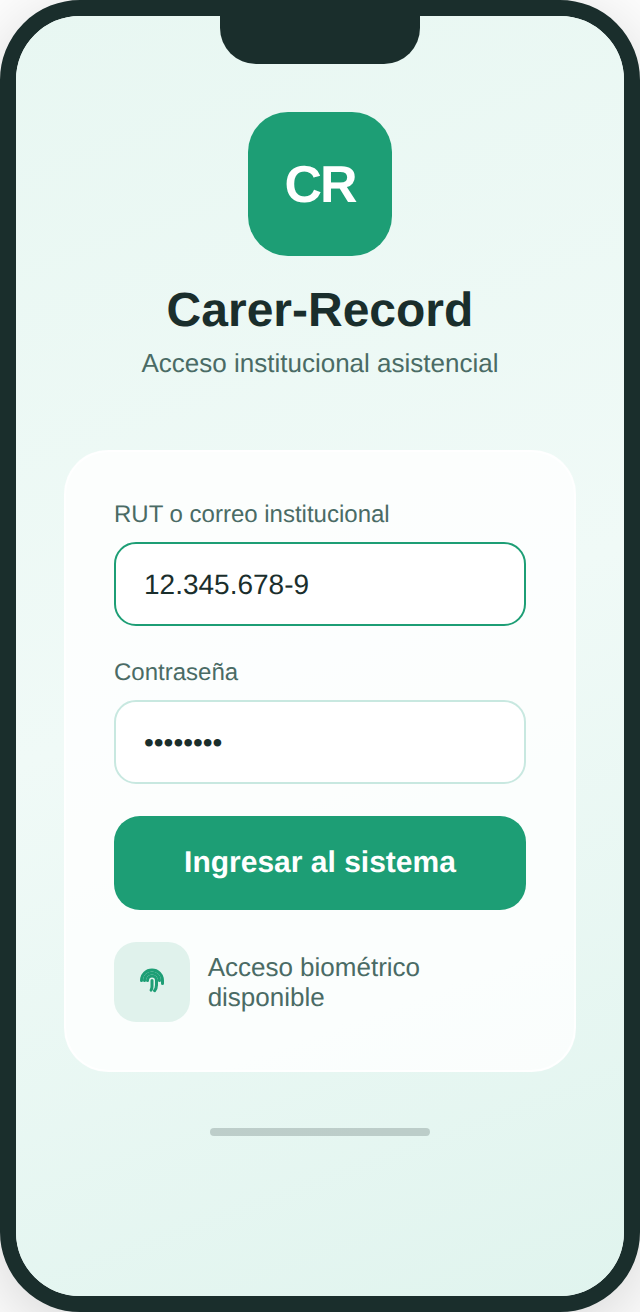
\includegraphics[width=0.2\textwidth]{Imagenes/vista1_autenticacion.png}
    \caption{Vista 1: Autenticación y acceso}
    \label{fig:vista1_autenticacion}
\end{figure}

\subsubsection*{Vista 2: Perfil del paciente activo y línea de tiempo} ~

La Figura~\ref{fig:vista2_timeline} presenta la vista central del sistema y la más crítica para el cambio de turno. Muestra el identificador simbólico del paciente activo, la información mínima del caso y la bitácora cronológica de eventos validados. Cada evento se presenta con su marca temporal, categoría y descripción, permitiendo al médico entrante leer el contexto completo del caso mediante desplazamiento vertical.

\begin{figure}[H]
    \centering
    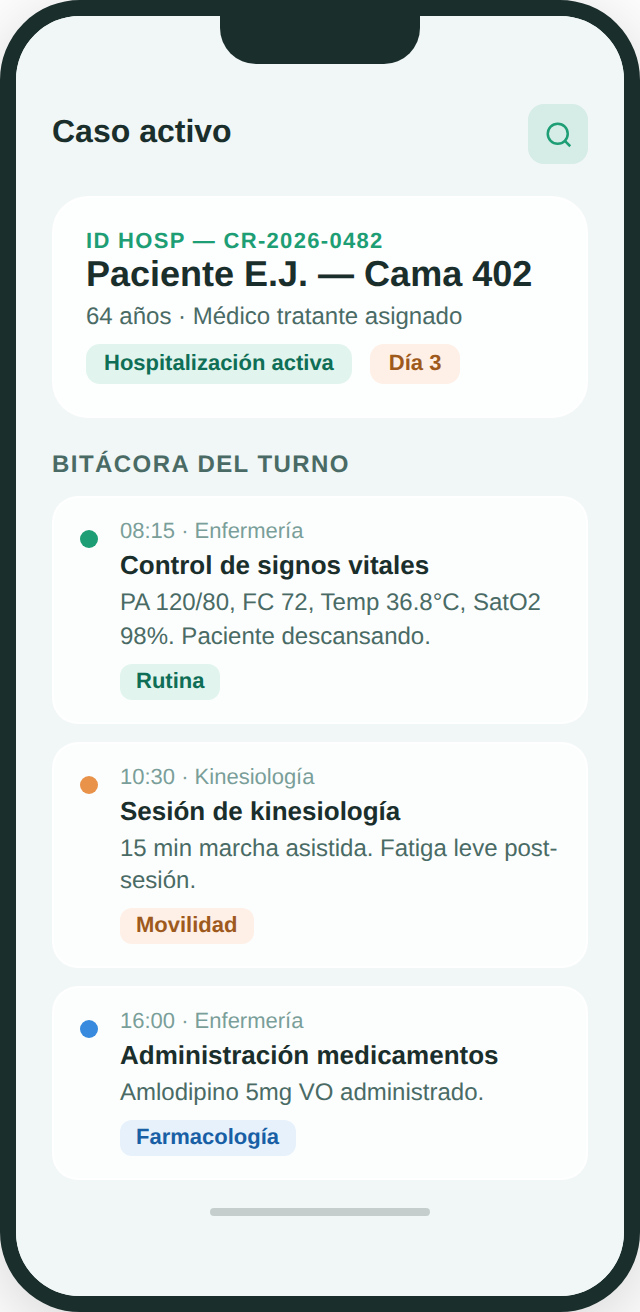
\includegraphics[width=0.2\textwidth]{Imagenes/vista2_linea_de_tiempo.png}
    \caption{Vista 2: Perfil del paciente activo y línea de tiempo}
    \label{fig:vista2_timeline}
\end{figure}

\subsubsection*{Vista 3: Captura de evento por audio o texto} ~

La Figura~\ref{fig:vista3_captura} presenta la vista para registrar un nuevo evento. Ofrece dos opciones de entrada claramente diferenciadas: grabación de audio mediante un botón de gran área táctil y un campo de texto para digitación directa. Las sugerencias de categoría que aparecen en la maqueta histórica no forman parte de los requisitos V4.

\begin{figure}[H]
    \centering
    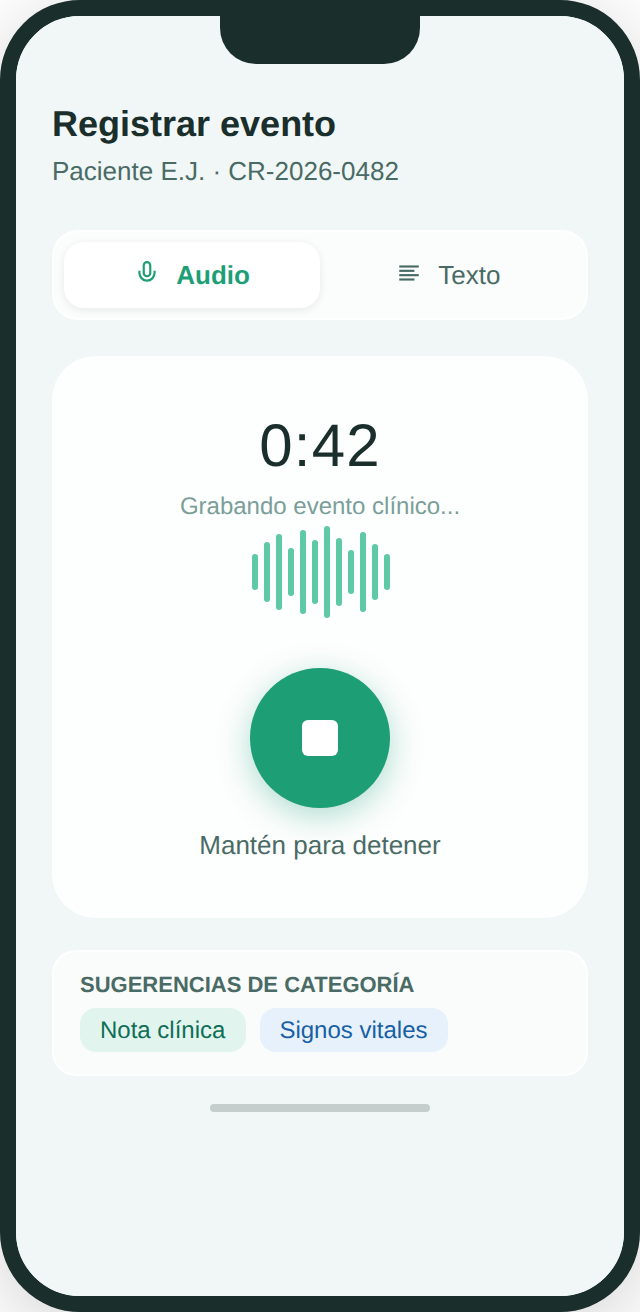
\includegraphics[width=0.2\textwidth]{Imagenes/vista3_captura_evento.png}
    \caption{Vista 3: Captura de evento por audio o texto}
    \label{fig:vista3_captura}
\end{figure}

\subsubsection*{Vista 4: Validación Human-in-the-Loop} ~

La validación con intervención humana (Human-in-the-Loop, HITL) mantiene a la persona autora en control de la revisión del contenido asistido.

La Figura~\ref{fig:vista4_validacion} es una maqueta histórica de revisión. Su transcripción y campos editables ilustran la revisión de contenido; las categorías y el porcentaje de confianza visibles son elementos gráficos históricos, no capacidades requeridas ni mediciones del sistema.

\begin{figure}[H]
    \centering
    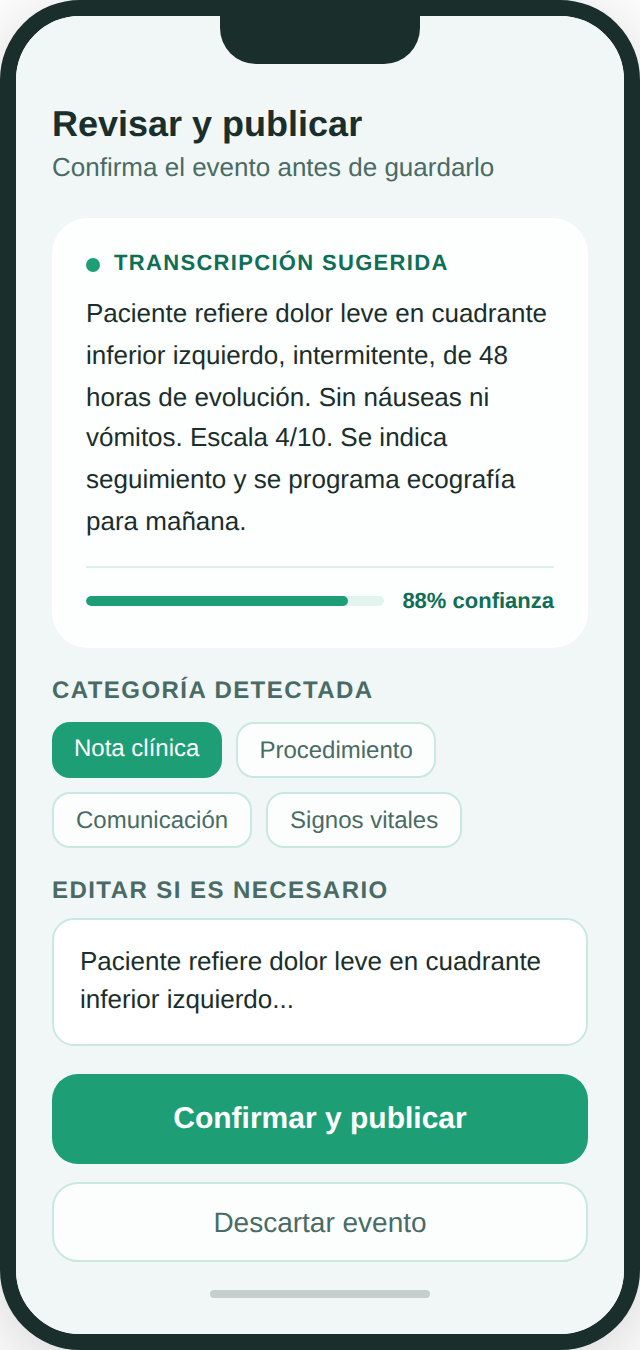
\includegraphics[width=0.2\textwidth]{Imagenes/vista4_validacion.png}
    \caption{Vista 4: Validación Human-in-the-Loop}
    \label{fig:vista4_validacion}
\end{figure}

\subsubsection*{Vista 5: Resumen de período para revisión} ~

La Figura~\ref{fig:vista5_borrador} es una maqueta histórica de resumen. Para el diseño V4, la vista representa la consulta y revisión de un resumen de eventos y notas de un período seleccionado; no supone publicarlo, copiarlo a la FCE ni cerrar un turno. La imagen histórica muestra un control de cierre de turno, que queda fuera del alcance V4 y no representa una función comprometida.

\begin{figure}[H]
    \centering
    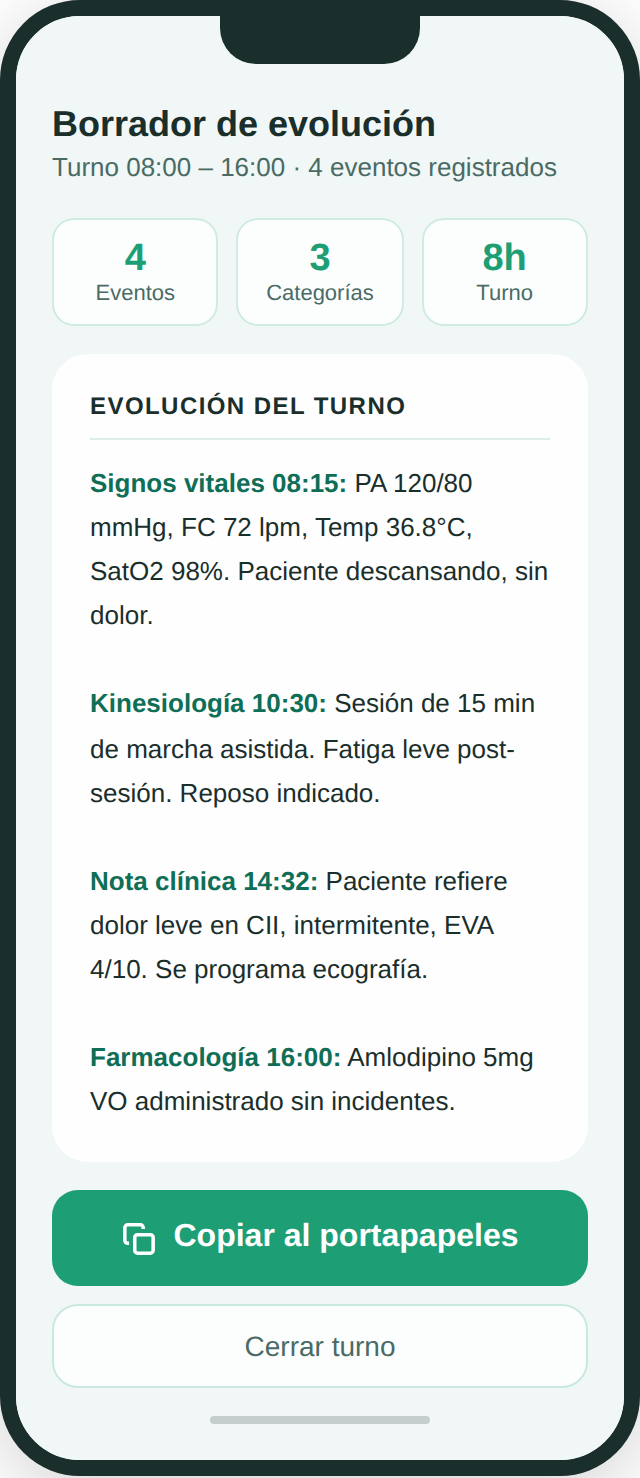
\includegraphics[width=0.2\textwidth]{Imagenes/vista5_borrador_evolucion.png}
    \caption{Vista 5: Resumen de período para revisión (maqueta histórica)}
    \label{fig:vista5_borrador}
\end{figure}

  Las maquetas descritas sirven como referencia visual para los recorridos de usabilidad; sus controles históricos no amplían el alcance funcional V4.

\subsection{Protocolo de test de usabilidad}

El protocolo propone evaluar si los recorridos de Carer-Record permiten al personal asistencial consultar contexto autorizado, registrar notas propias y revisar la asistencia y los resúmenes de período. La evaluación emplea datos sintéticos y no se afirma como ejecutada.

\subsubsection*{Objetivos del test} ~

El test busca observar la completitud de las tareas, el tiempo empleado, los errores y la comprensión de las vistas. También recoge la percepción general de usabilidad para orientar iteraciones de diseño. Los indicadores y umbrales descritos son criterios propuestos para esta evaluación, no resultados ni requisitos funcionales.

\subsubsection*{Perfil de participantes} ~

Se propone invitar a un mínimo de cinco participantes que correspondan al perfil de personal asistencial: médico tratante, médico de turno o profesional de enfermería con al menos un año de experiencia hospitalaria y uso habitual de smartphone. La participación es voluntaria y requiere consentimiento informado antes de comenzar. Este perfil no implica que se hayan reclutado o evaluado participantes.

\subsubsection*{Tareas a evaluar} ~

El Cuadro~\ref{tab:tareas_test_usabilidad} define seis tareas para recorrer el acceso, la consulta, el registro y la revisión de asistencia. Los tiempos son objetivos orientativos para observar el recorrido; no son garantías de rendimiento ni condiciones de aceptación del producto.

\begin{table}[H]
\caption{Tareas propuestas para el test de usabilidad}
\label{tab:tareas_test_usabilidad}
\begin{tabularx}{\textwidth}{|l|X|X|c|}
\hline
\textbf{N} & \textbf{Tarea} & \textbf{Criterio observable} & \textbf{Tiempo objetivo} \\
\hline
T-01 & Iniciar sesión y abrir una hospitalización sintética autorizada. & Se muestra el contexto permitido; un acceso sin autorización es denegado. & 30 s \\
\hline
T-02 & Consultar información de la FCE simulada y notas propias en la bitácora. & Se identifican las procedencias y el orden temporal de la información. & 2 min \\
\hline
T-03 & Redactar y confirmar una nota mediante texto. & La nota revisada queda asociada a la persona autora y a la hospitalización. & 60 s \\
\hline
T-04 & Dictar una nota, revisar la transcripción local y corregirla antes de confirmar. & Solo el texto revisado y confirmado queda registrado. & 60 s \\
\hline
T-05 & Solicitar asistencia de redacción y aceptar, editar o descartar la propuesta. & La decisión corresponde a la persona y el texto de origen no se sustituye automáticamente. & 90 s \\
\hline
T-06 & Seleccionar un período con varios eventos y notas y revisar su resumen. & El resumen identifica el período y sus fuentes, y no se publica como nota ni se escribe en la FCE. & 45 s \\
\hline
\end{tabularx}
\end{table}

\subsubsection*{Métricas y criterios de iteración} ~

Para cada tarea se propone registrar:

\begin{itemize}
    \item \textit{Completitud:} proporción de participantes que completa la tarea sin ayuda. Una completitud inferior al 80\% se propone como señal para revisar el diseño de esa tarea.
    \item \textit{Tiempo:} duración observada comparada con el objetivo orientativo del cuadro. Un promedio que supere el objetivo en más de 50\% se propone como señal para revisar el recorrido, no como incumplimiento del producto.
    \item \textit{Errores:} tipo y cantidad, distinguiendo errores recuperables de errores bloqueantes que requieren ayuda o impiden terminar.
    \item \textit{Usabilidad percibida:} aplicación del cuestionario System Usability Scale (SUS) de diez ítems al terminar; un resultado inferior a 70 puntos se propone como señal para iterar la interfaz~\cite{ref_brooke_sus}.
\end{itemize}

Los umbrales orientan decisiones de diseño y deben interpretarse junto con las observaciones y condiciones de aplicación; no acreditan por sí mismos la aceptación del producto. Una nueva ronda puede evaluar los cambios introducidos. Esta evaluación de usabilidad no sustituye la verificación técnica ni una revisión clínica diferenciada del contenido generado.

\subsubsection*{Protocolo de aplicación} ~

La prueba se propone en formato presencial, con una persona moderadora. Tras obtener el consentimiento, se entrega un escenario sintético y se permite que cada participante complete las tareas sin instrucciones sobre cómo usar la interfaz. La persona moderadora observa y registra pasos, tiempos y errores, e interviene solo si existe bloqueo o si la persona solicita detener la prueba. No se requiere grabar audio o video; cualquier registro adicional exige consentimiento explícito.

El escenario presenta a una persona asistencial que necesita consultar una hospitalización autorizada, revisar la FCE simulada y las notas propias, registrar contexto mediante texto y dictado, revisar una propuesta de redacción y generar un resumen de un período seleccionado. El resumen se revisa en Carer-Record y no se copia ni se escribe en la ficha oficial. El intervalo seleccionado no representa un turno.

Al terminar, se propone una entrevista breve sobre los pasos más confusos, los cambios sugeridos, la diferencia entre la FCE y las notas propias y si la persona usaría el sistema en su trabajo. La ejecución y sus resultados se documentarán si la evaluación se realiza; este protocolo no informa resultados.

\newpage

\section{Requisitos del sistema}

\subsection{Requisitos Funcionales}

Los RF definen el comportamiento esperado del sistema y las capacidades que debe ofrecer al personal asistencial. Se expresan con independencia del avance del prototipo; su grado de cumplimiento se analiza posteriormente en la sección de verificación y validación.

\subsubsection*{\textbf{RF1} - Identificación Mínima Segura}

El sistema debe permitir la apertura y gestión de un caso clínico mediante un identificador único de hospitalización, junto con los datos mínimos de contexto, ubicación y alertas críticas. Para fines académicos, se utilizarán datos sintéticos o ficticios.

\subsubsection*{\textbf{RF2} - Captura Multimodal de Eventos}

El sistema debe proveer al personal asistencial la capacidad de ingresar hitos clínicos o comunicacionales de manera ágil, ya sea mediante la grabación nativa de audio desde el dispositivo móvil o a través de la digitación de texto libre.

\subsubsection*{\textbf{RF3} - Procesamiento Asistido por Inteligencia Artificial}

Al recibir un ingreso de audio, el sistema debe ejecutar ASR para generar una transcripción preliminar. Posteriormente, un LLM debe analizar el registro y sugerir una clasificación basada en categorías predefinidas.

\subsubsection*{\textbf{RF4} - Filtrado dinámico de privacidad}

Antes de enviar registros a un servicio externo de IA, el sistema debe ejecutar reconocimiento de entidades nombradas (NER) para detectar y reemplazar IPS por tokens genéricos, reduciendo el riesgo de identificación de personas.

\subsubsection*{\textbf{RF5} - Validación clínica obligatoria}

El sistema debe bloquear la publicación automática de cualquier contenido generado por la IA, requiriendo un estado de revisión intermedio. El profesional deberá verificar, editar si es necesario, y confirmar explícitamente el evento, asumiendo la autoría clínica del registro.

\subsubsection*{\textbf{RF6} - Estructuración Inmutable de Metadatos}

Tras la validación, el sistema debe asignar automáticamente a cada evento una marca temporal del servidor y el identificador del autor, garantizando la trazabilidad del dato.

\subsubsection*{\textbf{RF7} - Construcción de Bitácora Cronológica}

El sistema debe organizar los eventos confirmados en una línea de tiempo interactiva y centralizada por paciente, permitiendo que cualquier profesional autorizado del equipo entrante visualice el historial completo de los turnos previos.

\subsubsection*{\textbf{RF8} - Síntesis Automatizada de Jornada (Cero Doble Trabajo)}

A petición del usuario, el sistema debe compilar los eventos registrados durante un turno y generar un documento estructurado denominado "Borrador de Evolución". Este borrador debe estar diseñado para ser copiado y pegado manualmente por el médico en la Ficha Clínica Electrónica oficial de la institución.

\subsubsection*{\textbf{RF9} - Cierre de ciclo hospitalario}

El sistema debe permitir declarar el alta médica. Esta acción debe dejar la bitácora en modo de solo lectura y bloquear nuevos ingresos para resguardar la integridad del historial.

\subsubsection*{\textbf{RF10} - Integración hospitalaria simulada}

El sistema debe permitir simular la integración con sistemas hospitalarios mediante la importación de recursos FHIR o mensajes HL7v2 con datos sintéticos. Los recursos recibidos deben validarse, normalizarse al modelo interno y quedar disponibles para su consulta en Carer-Record, sin requerir acceso a infraestructura ni datos clínicos reales.

\subsection{Requisitos No Funcionales}

Los requisitos no funcionales (RNF) establecen propiedades de calidad y restricciones transversales del producto, con independencia de la tecnología usada para implementarlas.

\subsubsection*{\textbf{RNF-01} - Acceso restringido y diferenciación de capacidades}

El acceso debe limitarse según las atribuciones vigentes, el ámbito institucional aplicable y, para la consulta clínica del personal asistencial, la relación asistencial con la hospitalización. Las capacidades disponibles deben diferenciarse según la autorización efectiva de cada persona.

\subsubsection*{\textbf{RNF-02} - Confidencialidad y privacidad}

La información debe protegerse durante su transmisión, almacenamiento y procesamiento. El procesamiento de capacidades asistidas no debe enviar contenido clínico a proveedores externos de inteligencia artificial.

\subsubsection*{\textbf{RNF-03} - Integridad de la información}

El sistema debe preservar la procedencia de la información, distinguir el contenido proveniente de fuentes externas del contenido propio o generado y prevenir duplicados y modificaciones no autorizadas.

\subsubsection*{\textbf{RNF-04} - Trazabilidad}

Las operaciones y el contenido registrado deben conservar metadatos suficientes para identificar procedencia, autoría, tiempos relevantes y operaciones realizadas, según corresponda.

\subsubsection*{\textbf{RNF-05} - Seguridad del contenido asistido}

El contenido asistido no debe incorporar antecedentes no presentes en sus fuentes ni formular diagnósticos. No debe publicarse automáticamente y debe quedar sujeto a revisión humana antes de cualquier uso como nota.

\subsubsection*{\textbf{RNF-06} - Usabilidad y baja carga cognitiva}

La interfaz móvil debe facilitar las tareas principales del personal asistencial con una presentación clara y una carga cognitiva reducida, sin imponer un modo de interacción no sustentado por el contexto de uso.

\subsubsection*{\textbf{RNF-07} - Rendimiento operativo}

El rendimiento de las operaciones relevantes debe ser compatible con las tareas previstas y sus criterios de aceptación. Debe evaluarse mediante mediciones reproducibles en dispositivos representativos del entorno objetivo e informarse con sus condiciones de prueba, sin presuponer umbrales no medidos.

\subsubsection*{\textbf{RNF-08} - Interoperabilidad}

Las interfaces de intercambio deben definir contratos explícitos para las fuentes integradas y permitir mapear la información pertinente al modelo del sistema. La selección de estándares debe responder al contrato de cada integración y no presupone un estándar único obligatorio.

\subsubsection*{\textbf{RNF-09} - Manejo de fallos}

Los fallos de una operación deben preservar las fuentes de información y no impedir tareas independientes que puedan continuar de forma segura. La recuperación ante fallos nunca debe omitir controles de autorización ni revisión humana.

\subsubsection*{\textbf{RNF-10} - Retención mínima}

Los artefactos temporales deben conservarse solo durante el tiempo necesario para completar su propósito y eliminarse conforme a la política de retención aplicable. La política debe contemplar los residuos de operaciones interrumpidas.

\subsection{Requisitos de Interfaces}

Los requisitos de interfaces definen las interacciones entre Carer-Record, el personal asistencial y las fuentes de datos clínicos. La Tabla~\ref{tab:eventos_externos} resume los eventos que ingresan al sistema, mientras que la Tabla~\ref{tab:respuestas_sistema} describe las respuestas esperadas. Ambas tablas expresan contratos lógicos y no obligan a utilizar una tecnología específica.

\begin{table}[H]
    \caption{Eventos externos}
    \label{tab:eventos_externos}
    \begin{tabularx}{\textwidth}{|l|X|X|X|X|}
        \hline
        \textbf{Evento} & \textbf{Descripción} & \textbf{Iniciador} & \textbf{Parámetros} & \textbf{Respuesta} \\
        \hline
        Autenticación de personal clínico & Solicitud de acceso al sistema móvil para verificar la identidad y determinar los permisos del profesional. & Personal asistencial & Credenciales institucionales o una sesión previamente autorizada. & Validación de acceso clínico \\
        \hline
        Integración hospitalaria simulada & Recepción de un caso clínico y sus antecedentes desde un sistema hospitalario simulado. & Simulador de SIH/FCE & Recursos FHIR o mensajes HL7v2 con datos sintéticos. & Resultado de validación, normalización y carga \\
        \hline
        Consulta de bitácora del paciente & El profesional solicita el perfil clínico activo y la línea de tiempo de hitos. & Personal asistencial & Identificador de hospitalización y sesión válida. & Despliegue de bitácora cronológica \\
        \hline
        Envío de hito asistencial & Transmisión de una nota de texto o una grabación de voz desde el dispositivo móvil. & Personal asistencial & Identificador de hospitalización, audio o texto y sesión válida. & Presentación de borrador para revisión \\
        \hline
        Confirmación y registro de evento & Acción explícita mediante la cual el profesional revisa y aprueba el contenido. & Personal asistencial & Identificador del borrador, texto final y categoría confirmada. & Registro trazable y publicación \\
        \hline
        Solicitud de borrador de evolución & Petición para consolidar los hitos validados de un turno. & Personal asistencial & Identificador de hospitalización y rango del turno. & Entrega de síntesis de evolución \\
        \hline
        Cierre de caso por alta médica & Declaración del término de la hospitalización y bloqueo de nuevos registros. & Personal asistencial & Identificador de hospitalización, confirmación y sesión válida. & Cierre de bitácora \\
        \hline
    \end{tabularx}
\end{table}

\begin{table}[H]
    \caption{Respuestas del sistema}
    \label{tab:respuestas_sistema}
    \begin{tabularx}{\textwidth}{|l|X|X|}
        \hline
        \textbf{Respuesta} & \textbf{Descripción} & \textbf{Parámetros} \\
        \hline
        Validación de acceso clínico & El sistema verifica la identidad, determina permisos y establece una sesión. & Resultado de autenticación, sesión y permisos asignados. \\
        \hline
        Resultado de validación, normalización y carga & El sistema informa los recursos aceptados o rechazados, registra el caso normalizado y habilita su seguimiento. & Estado de la ingesta, identificador del caso y errores detectados. \\
        \hline
        Despliegue de bitácora cronológica & El sistema recupera y ordena los eventos disponibles del paciente. & Datos mínimos del paciente y lista cronológica de hitos. \\
        \hline
        Presentación de borrador para revisión & El sistema transcribe el audio cuando corresponda y presenta el texto para revisión humana. Las etapas de NER y clasificación se incorporarán antes de procesar IPS real. & Texto preliminar, categoría sugerida cuando esté disponible e identificador del borrador. \\
        \hline
        Registro trazable y publicación & El sistema almacena el evento validado, registra su autoría y actualiza la bitácora. & Confirmación de publicación y metadatos del evento. \\
        \hline
        Entrega de síntesis de evolución & El sistema consolida los hitos del turno en un texto revisable y copiable. & Borrador de evolución. \\
        \hline
        Cierre de bitácora & El sistema marca el término de la hospitalización e impide nuevos eventos. & Estado de cierre y confirmación de solo lectura. \\
        \hline
    \end{tabularx}
\end{table}

Los contratos muestran que toda acción clínica parte de una identidad válida y produce una respuesta observable. La integración hospitalaria se evalúa mediante un simulador y datos sintéticos, de modo que su comportamiento puede verificarse sin depender de un convenio ni de infraestructura clínica real. Las etapas de procesamiento inteligente aún deben completarse antes del prototipo final.

\subsection{Requisitos de ambiente}

El ambiente de Carer-Record debe permitir el desarrollo y la evaluación del sistema sin utilizar datos clínicos reales. Estos requisitos describen condiciones operativas y no una pila tecnológica obligatoria.

\subsubsection{Dispositivo móvil}

El dispositivo debe contar con micrófono, almacenamiento temporal suficiente para grabaciones y capacidad para ejecutar la interfaz de forma fluida. Cuando se utilice ASR local, el dispositivo deberá disponer de los recursos necesarios para almacenar y ejecutar el modelo seleccionado.

\subsubsection{Servicios de aplicación}

El servicio central debe operar en una infraestructura con conectividad cifrada, gestión de secretos, respaldo y recuperación. Su capacidad de procesamiento debe dimensionarse a partir de mediciones de concurrencia, tamaño de archivos y latencia, evitando fijar requisitos de hardware antes de contar con resultados experimentales.

\subsubsection{Persistencia y archivos}

Los datos estructurados y los archivos de audio deben almacenarse en repositorios separados, con control de acceso, cifrado, retención definida y respaldo verificable. Los ambientes de desarrollo, prueba y eventual producción deben permanecer aislados.

\subsubsection{Datos de prueba e interoperabilidad}

La evaluación académica utilizará datos sintéticos para simular el intercambio con un SIH o una FCE. Los recursos provenientes del simulador deberán ajustarse a contratos FHIR o HL7v2, validarse y normalizarse antes de incorporarse al modelo interno. La conexión con infraestructura hospitalaria real y su certificación institucional no forman parte de Hito 3~\cite{hl7chile_clips}.


\newpage

\section{Arquitectura del sistema}

La arquitectura de solución de Carer-Record separa la interacción móvil, la consulta autorizada, la captura de notas y el procesamiento local. Esta distribución delimita responsabilidades y favorece la evolución independiente de sus componentes~\cite{arch_patterns_health}.

Flutter proporciona la aplicación móvil. Supabase aporta Auth, PostgreSQL con RLS, PostgREST, RPC y Edge Functions; una pasarela autorizada media la consulta a fuentes hospitalarias. El ASR y la asistencia de redacción y resumen se ejecutan en el dispositivo. El audio y la transcripción no confirmada no salen de este; las notas confirmadas sí se persisten en el backend.

La integración se plantea mediante una pasarela autorizada y contratos explícitos con las fuentes. La fuente de demostración es una FCE simulada con FHIR R4 en Docker y datos sintéticos; esta configuración no representa una conexión productiva. El estándar de la demostración no limita los contratos de otras fuentes integradas. Carer-Record no escribe en la FCE.

\subsection{Contexto del sistema y actores externos}

La Figura~\ref{fig:diagrama_de_contexto} delimita Carer-Record como una unidad y muestra las entidades externas que interactúan con la solución.

\begin{figure}[H]
    \centering
    \resizebox{0.95\textwidth}{!}{%
    \begin{tikzpicture}[
        actor/.style={draw, rounded corners, align=center, minimum width=3.8cm, minimum height=1.4cm, fill=gray!12},
        system/.style={draw=blue!60!black, very thick, rounded corners, align=center, minimum width=4.2cm, minimum height=2cm, fill=blue!8},
        flow/.style={-{Latex[length=3mm]}, thick}
    ]
        \node[actor] (clinical) {Personal asistencial\\Médicos y enfermería};
        \node[system, right=4.2cm of clinical] (carer) {Carer-Record\\Sistema de trazabilidad asistencial};
        \node[actor, right=4.2cm of carer] (source) {FCE simulada\\FHIR R4 en Docker, datos sintéticos};

        \draw[flow] ([yshift=4mm]clinical.east) -- node[above, align=center]{Consulta, registra notas\\y revisa propuestas} ([yshift=4mm]carer.west);
        \draw[flow] ([yshift=-4mm]carer.west) -- node[below, align=center]{Contexto autorizado,\\bitácora y resúmenes} ([yshift=-4mm]clinical.east);
        \draw[flow] (source.west) -- node[above, align=center]{Consulta mediante\\pasarela autorizada} (carer.east);
    \end{tikzpicture}%
    }
    \caption{Contexto y fronteras externas de Carer-Record}
    \label{fig:diagrama_de_contexto}
\end{figure}

El personal asistencial consulta información autorizada, registra notas propias y revisa propuestas. La aplicación accede a fuentes hospitalarias mediante una pasarela autorizada, no directamente. La demostración utiliza la FCE simulada FHIR R4 en Docker con datos sintéticos. Carer-Record no escribe en la FCE.

\subsection{Arquitectura de componentes}

La Figura~\ref{fig:diagrama_arquitectura} presenta la arquitectura implementada y diferencia los componentes propios de Carer-Record de los sistemas hospitalarios externos.

\begin{figure}[H]
    \centering
    \resizebox{\textwidth}{!}{%
    \begin{tikzpicture}[
        component/.style={draw, rounded corners, align=center, minimum width=3cm, minimum height=1.2cm, fill=blue!8},
        service/.style={draw, rounded corners, align=center, minimum width=2.7cm, minimum height=1.1cm, fill=green!10},
        data/.style={draw, rounded corners, align=center, minimum width=2.7cm, minimum height=1.1cm, fill=violet!10},
        external/.style={draw, dashed, rounded corners, align=center, minimum width=3cm, minimum height=1.2cm, fill=gray!10},
        boundary/.style={draw=blue!50!black, thick, rounded corners, inner sep=8mm},
        flow/.style={-{Latex[length=2.5mm]}, thick}
    ]
        \node[component] (flutter) {Aplicación móvil\\Flutter};
        \node[component, right=2.2cm of flutter] (api) {API y lógica de negocio\\FastAPI cloud};
        \node[service, above right=1.1cm and 2.1cm of api] (stt) {Servicio ASR\\Transcripción};
        \node[service, below right=1.1cm and 2.1cm of api] (llm) {Servicio LLM\\Clasificación y síntesis};
        \node[data, right=2.2cm of stt] (auth) {Supabase Auth\\Identidad y sesión};
        \node[data, right=2.2cm of api] (db) {PostgreSQL\\Datos estructurados};
        \node[data, right=2.2cm of llm] (storage) {Supabase Storage\\Archivos privados};
        \node[service, right=2.2cm of db] (interop) {Adaptadores de interoperabilidad\\FHIR / HL7v2};
        \node[external, right=2.4cm of interop] (simulator) {Simulador de SIH/FCE\\Datos sintéticos};

        \node[boundary, fit=(flutter)(api)(stt)(llm)(auth)(db)(storage)(interop), label=above:{Frontera de Carer-Record}] (system) {};

        \draw[flow] (flutter) -- node[above]{Operaciones clínicas} (api);
        \draw[flow] ([yshift=3mm]flutter.east) to[bend left=25] node[above]{Credenciales} (auth.west);
        \draw[flow] (auth.west) to[bend left=18] node[below]{Sesión} ([yshift=-3mm]flutter.east);
        \draw[flow] (api) -- (stt);
        \draw[flow] (api) -- (llm);
        \draw[flow] (api) -- (auth);
        \draw[flow] (api) -- (db);
        \draw[flow] (api) -- (storage);
        \draw[flow] (simulator.west) -- node[above]{Datos sintéticos} (interop.east);
        \draw[flow] (interop.west) -- node[above]{Datos normalizados} (db.east);
    \end{tikzpicture}%
    }
    \caption{Arquitectura de componentes implementada en Carer-Record}
    \label{fig:diagrama_arquitectura}
\end{figure}

La aplicación Flutter concentra la interacción con el personal asistencial. FastAPI aplica autorización y reglas de negocio antes de acceder a los servicios administrados. Supabase Auth emite la sesión; PostgreSQL mantiene los datos estructurados; y Storage conserva archivos privados. Los servicios ASR y LLM se invocan desde la API para impedir que la aplicación móvil acceda directamente a credenciales de infraestructura. Los adaptadores de interoperabilidad reciben recursos FHIR o mensajes HL7v2 sintéticos, los normalizan y permiten comprobar el intercambio con un sistema hospitalario simulado dentro del alcance de Hito 3.

La separación por componentes favorece bajo acoplamiento, despliegue independiente de los procesos de IA y una frontera clara para aplicar seguridad. La implementación utiliza módulos lógicos coordinados por FastAPI, sin imponer un microservicio independiente para cada responsabilidad~\cite{arch_patterns_health}.

\subsection{Enumeración y funcionalidad lógica de los módulos}

La arquitectura se organiza en los seis módulos lógicos resumidos en la Tabla~\ref{tab:modulos_arquitectura}. Los módulos representan responsabilidades implementadas sobre los componentes descritos y no servicios necesariamente desplegados por separado.

\begin{table}[H]
    \caption{Módulos lógicos de la arquitectura implementada}
    \label{tab:modulos_arquitectura}
    \begin{tabularx}{\textwidth}{|l|X|X|}
        \hline
        \textbf{Módulo} & \textbf{Responsabilidad} & \textbf{Componentes principales} \\
        \hline
        M1: Captura e ingesta & Capturar texto o audio e importar recursos clínicos sintéticos desde sistemas hospitalarios simulados. & Flutter, FastAPI, servicio ASR y adaptadores FHIR/HL7v2. \\
        \hline
        M2: Privacidad & Detectar y enmascarar IPS antes de invocar servicios externos de IA. & FastAPI y motor NER. \\
        \hline
        M3: Procesamiento & Clasificar eventos y generar borradores a partir de información validada y acotada. & Servicio LLM y reglas de generación. \\
        \hline
        M4: Gobernanza & Gestionar revisión, corrección, aprobación, rechazo y cierre de eventos. & FastAPI y aplicación Flutter. \\
        \hline
        M5: Identidad & Autenticar usuarios, validar sesiones y aplicar permisos por rol e institución. & Supabase Auth y FastAPI. \\
        \hline
        M6: Auditoría & Registrar acciones críticas y conservar metadatos suficientes para su auditoría. & FastAPI y PostgreSQL. \\
        \hline
    \end{tabularx}
\end{table}

M1 inicia tanto el flujo asistencial como el de interoperabilidad simulada y M4 controla su consolidación. M2 y M3 aíslan el tratamiento de privacidad del procesamiento generativo, mientras M5 y M6 operan transversalmente sobre el flujo completo.

\subsection{Matriz de requisitos funcionales y responsabilidad modular}

El Cuadro~\ref{tab:matriz_rf} relaciona los siete requisitos funcionales con los módulos responsables. Una marca indica responsabilidad de diseño, no grado de implementación ni resultado de verificación.

\begin{table}[H]
\caption{Trazabilidad entre requisitos funcionales y módulos}
\label{tab:matriz_rf}
\centering
\begin{tabularx}{\textwidth}{|X|c|c|c|c|c|c|}
\hline
\textbf{Requisito} & \textbf{M1} & \textbf{M2} & \textbf{M3} & \textbf{M4} & \textbf{M5} & \textbf{M6} \\
\hline
RF-01: Integración con fuentes de información hospitalaria & \checkmark & \checkmark & & & \checkmark & \checkmark \\
\hline
RF-02: Consulta del contexto clínico & & \checkmark & & & \checkmark & \checkmark \\
\hline
RF-03: Visualización de la bitácora asistencial & & \checkmark & & & \checkmark & \checkmark \\
\hline
RF-04: Registro de notas de contexto & & \checkmark & \checkmark & & \checkmark & \checkmark \\
\hline
RF-05: Transcripción de dictados & & & \checkmark & & & \checkmark \\
\hline
RF-06: Asistencia para la redacción & & & & \checkmark & & \checkmark \\
\hline
RF-07: Resúmenes asistidos & & \checkmark & & \checkmark & \checkmark & \checkmark \\
\hline
\end{tabularx}
\end{table}

M5 y M6 son transversales a las operaciones protegidas y al registro de procedencia y autoría. La matriz expresa la distribución prevista de responsabilidades; la evidencia de implementación y verificación se informa por separado.

\subsection{Especificaciones de los módulos críticos}

\subsubsection*{M1: Captura e ingesta}

La Tabla~\ref{tab:modulo_m1} especifica el punto de entrada de eventos clínicos.

\begin{table}[H]
    \caption{Especificación arquitectónica de M1}
    \label{tab:modulo_m1}
    \begin{tabularx}{\textwidth}{|l|X|}
        \hline
        \textbf{Atributo} & \textbf{Descripción} \\
        \hline
        Propósito & Recibir texto o audio desde Flutter e importar recursos clínicos sintéticos desde un sistema hospitalario simulado. \\
        \hline
        Flujo objetivo & Validar sesión y caso para la captura asistencial; validar y normalizar recursos FHIR o mensajes HL7v2 para la ingesta simulada; y asignar metadatos antes de persistir cada resultado. \\
        \hline
        Dependencias & Flutter, FastAPI, servicio ASR, adaptadores FHIR/HL7v2, PostgreSQL y Storage. \\
        \hline
        Restricciones & Validar formato y tamaño del audio, rechazar recursos clínicos inválidos, utilizar solo datos sintéticos y no confiar en identificadores enviados sin validación. \\
        \hline
    \end{tabularx}
\end{table}

M1 admite transcripción local o remota sin alterar el contrato del evento. Los audios remotos se conservan en Storage y la identidad del autor se obtiene de la sesión validada por FastAPI. En el flujo de interoperabilidad, los adaptadores transforman datos sintéticos al modelo interno antes de dejarlos disponibles para consulta.

\subsubsection*{M2: Privacidad y desidentificación}

La Tabla~\ref{tab:modulo_m2} define la barrera previa al procesamiento generativo.

\begin{table}[H]
    \caption{Especificación arquitectónica de M2}
    \label{tab:modulo_m2}
    \begin{tabularx}{\textwidth}{|l|X|}
        \hline
        \textbf{Atributo} & \textbf{Descripción} \\
        \hline
        Propósito & Detectar y reemplazar IPS antes de enviar texto a un LLM externo. \\
        \hline
        Flujo objetivo & Aplicar reglas y NER, conservar la relación de sustitución en un entorno protegido y entregar solo texto sanitizado a M3. \\
        \hline
        Dependencias & M1, motor NER y políticas institucionales de tratamiento de datos. \\
        \hline
        Restricciones & Medir precisión y exhaustividad con datos sintéticos antes de procesar información real. \\
        \hline
    \end{tabularx}
\end{table}

La separación de M2 evita que el proveedor generativo reciba identificadores innecesarios. Su procesamiento combina reglas y NER antes de entregar texto sanitizado a M3~\cite{nlp_ner_privacy}.

\subsubsection*{M3: Procesamiento cognitivo}

La Tabla~\ref{tab:modulo_m3} resume las restricciones aplicables a la clasificación y síntesis.

\begin{table}[H]
    \caption{Especificación arquitectónica de M3}
    \label{tab:modulo_m3}
    \begin{tabularx}{\textwidth}{|l|X|}
        \hline
        \textbf{Atributo} & \textbf{Descripción} \\
        \hline
        Propósito & Sugerir categorías y producir borradores de evolución a partir de eventos del turno. \\
        \hline
        Flujo objetivo & Recibir texto sanitizado, aplicar instrucciones acotadas y devolver una propuesta identificada como contenido generado. \\
        \hline
        Dependencias & M2, servicio LLM y catálogo de categorías. \\
        \hline
        Restricciones & No diagnosticar, no completar antecedentes ausentes y no publicar resultados automáticamente. \\
        \hline
    \end{tabularx}
\end{table}

M3 opera como asistencia y no como fuente autónoma de verdad clínica. La literatura evidencia errores residuales en la generación de resúmenes, lo que obliga a mantener revisión experta~\cite{rust2025}.

\subsubsection*{M4: Gobernanza y validación clínica}

La Tabla~\ref{tab:modulo_m4} describe el control HITL del ciclo de vida de cada evento.

\begin{table}[H]
    \caption{Especificación arquitectónica de M4}
    \label{tab:modulo_m4}
    \begin{tabularx}{\textwidth}{|l|X|}
        \hline
        \textbf{Atributo} & \textbf{Descripción} \\
        \hline
        Propósito & Exigir revisión, corrección y confirmación antes de consolidar contenido generado por IA. \\
        \hline
        Flujo objetivo & Recibir borrador, presentarlo como editable, registrar la decisión del profesional y publicar solo tras aprobación. \\
        \hline
        Dependencias & M3, M5, M6 y aplicación Flutter. \\
        \hline
        Restricciones & Impedir autoaprobación y distinguir claramente contenido preliminar de contenido confirmado. \\
        \hline
    \end{tabularx}
\end{table}

El flujo HITL mantiene la responsabilidad en el profesional y permite corregir errores previsibles de la IA antes de integrar un evento a la bitácora~\cite{lazaros2026}.

\subsubsection*{M5 y M6: Identidad y auditoría}

La Tabla~\ref{tab:modulos_m5_m6} reúne las responsabilidades transversales de control de acceso y trazabilidad.

\begin{table}[H]
    \caption{Especificación arquitectónica de M5 y M6}
    \label{tab:modulos_m5_m6}
    \begin{tabularx}{\textwidth}{|l|X|X|}
        \hline
        \textbf{Módulo} & \textbf{Propósito} & \textbf{Condición objetivo} \\
        \hline
        M5: Identidad & Autenticar, validar sesiones y aplicar permisos por rol e institución. & Supabase Auth emite la sesión y FastAPI valida cada operación protegida. \\
        \hline
        M6: Auditoría & Registrar actor, acción, recurso, resultado y marca temporal. & Los registros se protegen frente a cambios y se someten a una política de retención. \\
        \hline
    \end{tabularx}
\end{table}

Supabase Auth administra las sesiones y FastAPI valida el usuario y sus permisos antes de procesar operaciones clínicas. La auditoría registra las acciones críticas junto con el actor, el recurso, el resultado y la marca temporal.

\subsection{Conclusión del diseño de arquitectura}

La arquitectura implementada separa presentación, negocio, IA, interoperabilidad, identidad, persistencia y archivos. Flutter y FastAPI mantienen el flujo de interacción y negocio, Supabase centraliza autenticación, datos y almacenamiento privado, y los adaptadores FHIR/HL7v2 permiten simular la ingesta desde sistemas hospitalarios.

El diseño establece barreras explícitas: M2 precede a cualquier LLM externo, M4 impide la publicación automática y M5 junto con M6 controlan acceso y trazabilidad. La simulación permite verificar la integración sin datos ni infraestructura hospitalaria real. Esta estructura permite concentrar el trabajo restante en completar y validar las funciones clínicas del prototipo, sin requerir un cambio de infraestructura.


\newpage

\section{Revisión del prototipo}

\subsection{Alcance del prototipo parcial}

Hito 3 presenta un prototipo parcial orientado a comprobar la captura, procesamiento y consulta de eventos asistenciales desde una aplicación móvil, además de la integración simulada con sistemas hospitalarios mediante datos sintéticos. La arquitectura e infraestructura se encuentran implementadas sobre Flutter, FastAPI cloud y Supabase; el carácter parcial corresponde a las funcionalidades clínicas y actividades de validación que se completarán en Hito 4.

La Tabla~\ref{tab:infraestructura_implementada} resume los componentes que sostienen el prototipo.

\begin{table}[H]
    \caption{Infraestructura implementada para Carer-Record}
    \label{tab:infraestructura_implementada}
    \begin{tabularx}{\textwidth}{|l|X|X|}
        \hline
        \textbf{Área} & \textbf{Componente} & \textbf{Responsabilidad} \\
        \hline
        Aplicación móvil & Flutter & Interacción, captura de texto y audio y presentación de la bitácora. \\
        \hline
        Servicios & FastAPI cloud & API, reglas de negocio, autorización y coordinación de procesos de IA. \\
        \hline
        Identidad & Supabase Auth & Autenticación, sesión y emisión de credenciales de acceso. \\
        \hline
        Persistencia & PostgreSQL de Supabase & Datos clínicos sintéticos, usuarios, eventos y metadatos. \\
        \hline
        Archivos & Supabase Storage & Almacenamiento privado de audio y archivos asociados. \\
        \hline
        Interoperabilidad & Adaptadores FHIR/HL7v2 & Recepción y normalización de datos sintéticos desde un SIH/FCE simulado. \\
        \hline
    \end{tabularx}
\end{table}

La distribución concentra en FastAPI la lógica clínica y evita el acceso directo de Flutter a los datos sensibles. Supabase provee los servicios administrados de identidad, persistencia y archivos, reduciendo tareas operativas y manteniendo una frontera uniforme de seguridad.

\subsection{Recorridos funcionales y evidencia}

La revisión del prototipo describe las vistas de la aplicación desarrollada y los recorridos previstos: localizar una hospitalización autorizada, consultar información externa y notas propias, redactar o dictar una nota, revisar transcripción y asistencia de redacción, confirmar la nota y solicitar un resumen del período seleccionado. Esta descripción de la implementación no equivale a una prueba observada con participantes ni demuestra usabilidad, eficacia, seguridad, calidad, latencia o aceptación.

Los recorridos enlazan la consulta de la FCE con el registro de contexto y la asistencia local. La revisión distingue el contenido obtenido de la fuente, las notas confirmadas por su autor y los resúmenes derivados para consulta. La evidencia y las condiciones de evaluación de estos recorridos se documentan en la sección de verificación y validación.

La evidencia visual combina las cinco maquetas históricas de la sección de fabricación preliminar, que representan diseño, con una selección de capturas de la interfaz implementada. Las capturas documentan pantallas, no prueban por sí solas autorización, operación local efectiva de modelos ni calidad funcional. No se han realizado pruebas con participantes ni en producción. La demostración se limita a información sintética y no acredita aptitud para datos clínicos reales, integración productiva con una institución, seguridad hospitalaria productiva ni cumplimiento normativo garantizado.

La selección sigue algunos recorridos de la interfaz; las maquetas históricas se conservan en la sección de fabricación preliminar y no deben confundirse con estas capturas de implementación.

\subsubsection*{Acceso y consulta de hospitalizaciones}

La Figura~\ref{fig:impl-acceso} reúne las pantallas de autenticación y listado de hospitalizaciones.

\begin{figure}[H]
    \centering
    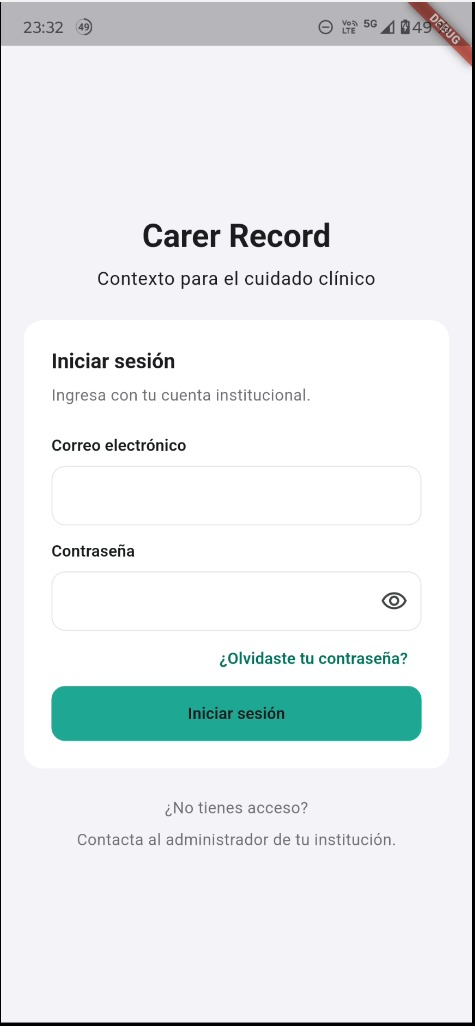
\includegraphics[width=0.45\textwidth]{Imagenes/app_autenticacion.jpeg}
    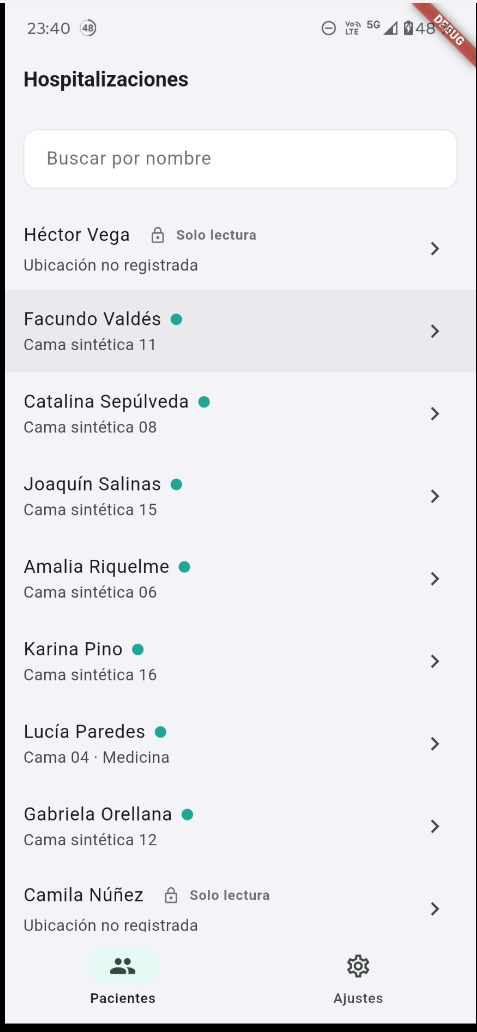
\includegraphics[width=0.45\textwidth]{Imagenes/app_hospitalizaciones.jpeg}
    \caption{Interfaz implementada: autenticación y hospitalizaciones (datos sintéticos).}
    \label{fig:impl-acceso}
\end{figure}

\subsubsection*{Consulta clínica y registro de contexto}

La Figura~\ref{fig:impl-ficha} reúne vistas de la ficha clínica. La Figura~\ref{fig:impl-nota} muestra la revisión de una nota dictada y su aparición en la bitácora.

\begin{figure}[H]
    \centering
    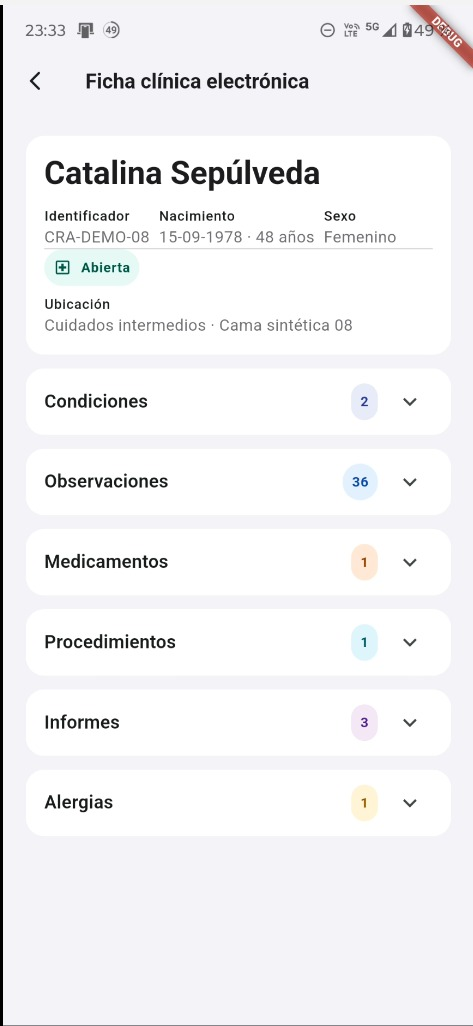
\includegraphics[width=0.45\textwidth]{Imagenes/app_ficha_clinica_general.jpeg}
    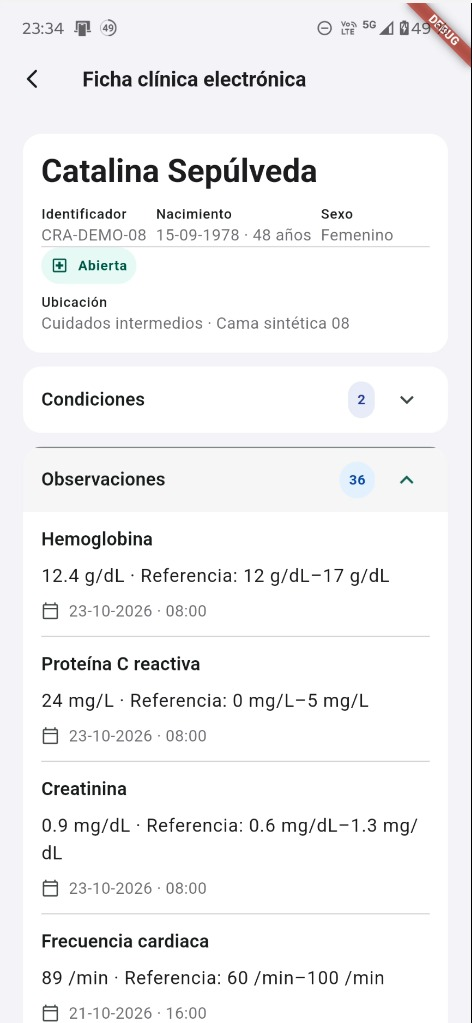
\includegraphics[width=0.45\textwidth]{Imagenes/app_ficha_clinica_observaciones.jpeg}
    \caption{Interfaz implementada: vistas de ficha clínica (datos sintéticos).}
    \label{fig:impl-ficha}
\end{figure}

\begin{figure}[H]
    \centering
    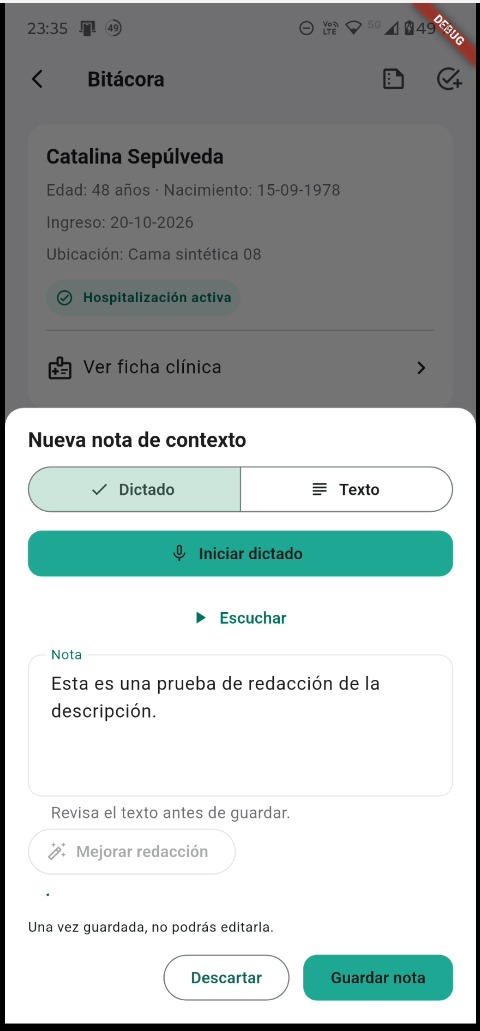
\includegraphics[width=0.45\textwidth]{Imagenes/app_nota_dictada_revision.jpeg}
    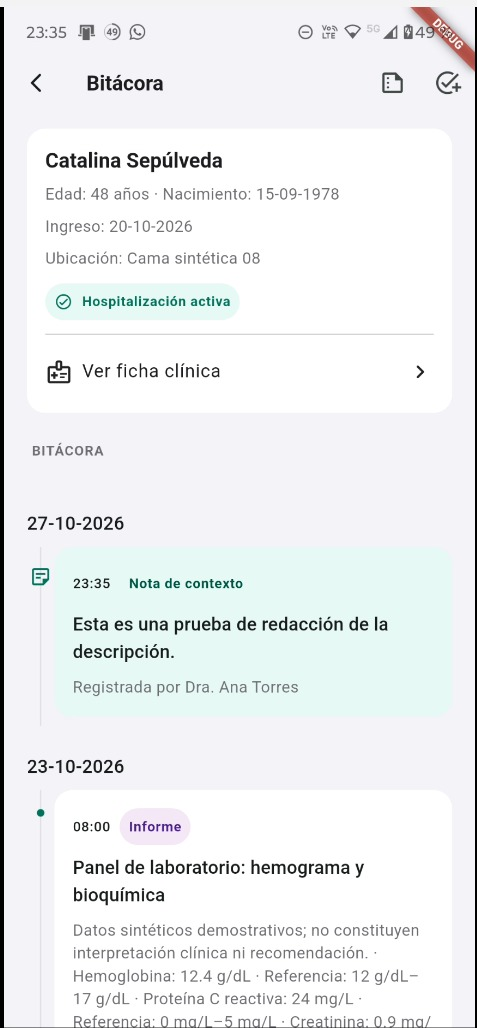
\includegraphics[width=0.45\textwidth]{Imagenes/app_bitacora_nota_confirmada.jpeg}
    \caption{Interfaz implementada: revisión de nota dictada y bitácora (datos sintéticos).}
    \label{fig:impl-nota}
\end{figure}

\subsubsection*{Configuración visible}

La Figura~\ref{fig:impl-configuracion} muestra la interfaz de configuración de permisos clínicos y la pantalla de modelos locales; no constituye evidencia de autorización efectiva ni de procesamiento local efectivo.

\begin{figure}[H]
    \centering
    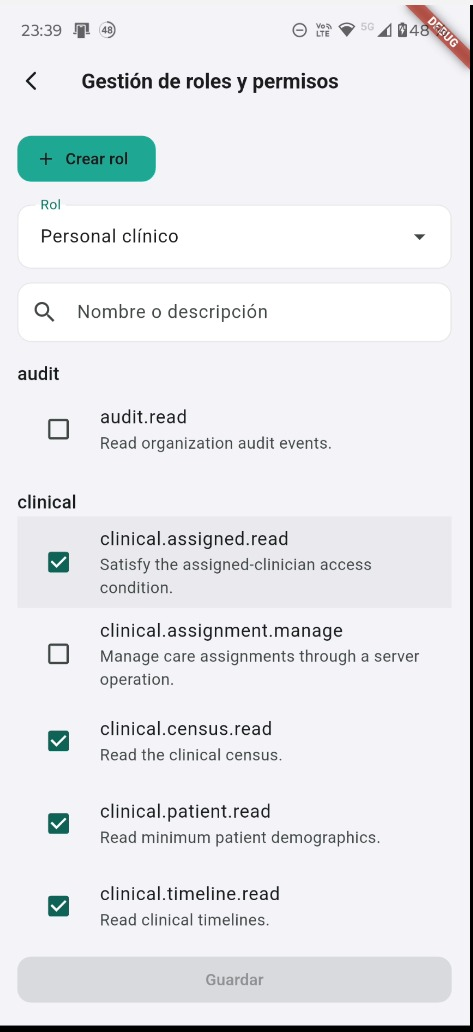
\includegraphics[width=0.45\textwidth]{Imagenes/app_roles_permisos_clinicos.jpeg}
    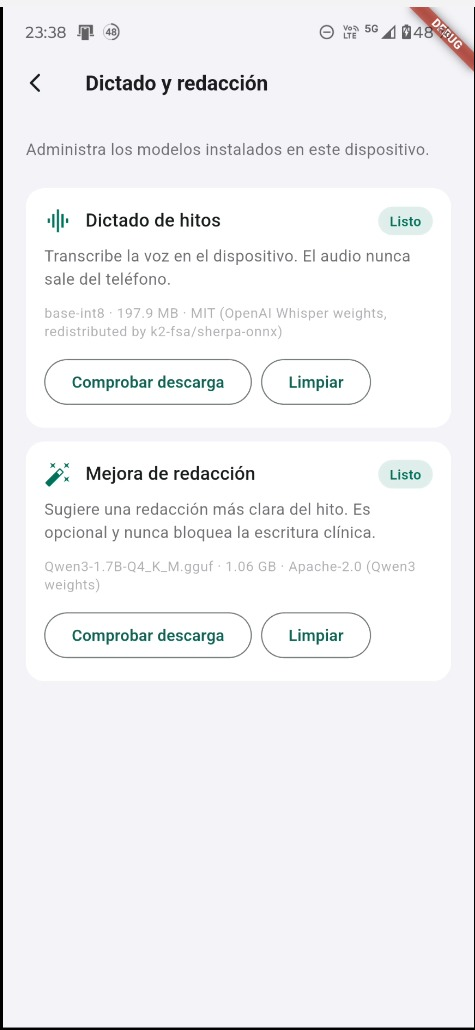
\includegraphics[width=0.45\textwidth]{Imagenes/app_modelos_locales.jpeg}
    \caption{Interfaz implementada: permisos clínicos y modelos locales (datos sintéticos).}
    \label{fig:impl-configuracion}
\end{figure}

\subsection{Límites de entrega y evidencia}

La entrega académica se delimita al alcance funcional descrito en los requisitos. La demostración utiliza datos sintéticos y no es apta para datos reales.

Quedan fuera del alcance la escritura en la FCE, la publicación de resúmenes, el alta o cierre de hospitalizaciones, la gestión de turnos y una operación offline completa. La consulta de la FCE se media mediante una pasarela autorizada; la FCE simulada FHIR R4 en Docker con datos sintéticos no representa un entorno hospitalario productivo.

La existencia de una maqueta o de un recorrido propuesto no constituye evidencia de implementación o validación. La matriz de verificación identifica evidencia que deberá registrarse; no se presuponen resultados, participantes, mediciones de rendimiento, evaluación clínica ni cumplimiento normativo garantizado.


\newpage

\section{Planificación del proyecto}

\subsection{Objetivo General (Goal)}

Diseñar y desarrollar una solución móvil que integre consulta autorizada de la FCE, bitácora de notas propias y asistencia local para fortalecer la trazabilidad y continuidad del contexto clínico durante la hospitalización, sin reemplazar ni escribir en el registro oficial.

\subsection{Objetivos Específicos}

Los objetivos específicos (OE) organizan el trabajo de diseño y desarrollo necesario para alcanzar el producto final descrito en este informe.

\begin{itemize}
    \item \textbf{OE1.} Desarrollar la integración con fuentes hospitalarias autorizadas mediante contratos explícitos y una pasarela de consulta, utilizando datos sintéticos en la demostración académica.

    \item \textbf{OE2.} Implementar la captura de notas por texto o dictado, la transcripción y asistencia de redacción locales, y los resúmenes revisables de eventos y notas para un período seleccionado.

    \item \textbf{OE3.} Diseñar e implementar la aplicación móvil y sus controles de acceso y trazabilidad para permitir la consulta y el registro de contexto según las atribuciones del personal.

\end{itemize}

\subsection{Actividades y Milestones}

El Cuadro~\ref{tab:actividades_milestones} concilia la planificación aplicable del libro de seguimiento con el alcance vigente del prototipo. Las fechas y responsables se conservan cuando corresponden a trabajo vigente. El porcentaje indica la meta prevista para la entrega de Hito 4 al 13-11-2026; no representa avance observado ni evidencia de cumplimiento.

\begin{table}[H]
\centering
\caption{Actividades y hitos aplicables del proyecto}
\label{tab:actividades_milestones}
\renewcommand{\arraystretch}{1.2}
\resizebox{\textwidth}{!}{%
\begin{tabular}{|p{5.8cm}|p{2.8cm}|l|l|p{4.4cm}|}
\hline
\textbf{Elemento} & \textbf{Responsable} & \textbf{Inicio} & \textbf{Término} & \textbf{Meta prevista Hito 4} \\
\hline
\textbf{A1.1} Análisis de sistemas y fuentes clínicas (OE1) & Ignacio Muñoz & 15-05-2026 & 15-06-2026 & 100\% \\
\hline
\textbf{A1.2} Diseño de integración hospitalaria mediante pasarela autorizada (OE1) & Francisco Castillo & 15-05-2026 & 15-07-2026 & 100\% \\
\hline
\textbf{RP1} Plataforma base e interoperabilidad & Carlos López & 15-05-2026 & 15-07-2026 & 100\% \\
\hline
\textbf{H1.1} Definición del flujo y criterios de interoperabilidad & Ignacio Muñoz & 15-06-2026 & 15-07-2026 & 100\% \\
\hline
\textbf{H1.2} Verificación inicial de integración & Ignacio Muñoz & 01-07-2026 & 30-07-2026 & 100\% \\
\hline
\textbf{A2.1} Diseño de procesamiento local y asistencia revisable (OE2) & Carlos López & 15-07-2026 & 15-10-2026 & 100\% \\
\hline
\textbf{RP2} Sistema de acceso y procesamiento revisable & Ignacio Muñoz & 15-07-2026 & 13-11-2026 & 100\% \\
\hline
\textbf{H2.1} Autenticación y flujo de revisión humana & Ignacio Muñoz & 15-07-2026 & 13-11-2026 & 100\% \\
\hline
\textbf{A3.1} Diseño de interfaces de usuario (OE3) & Sebastián Saavedra & 15-09-2026 & 15-10-2026 & 100\% \\
\hline
\textbf{A3.2} Implementación de autenticación (OE3) & Francisco Castillo & 15-10-2026 & 13-11-2026 & 100\% \\
\hline
\textbf{A3.3} Verificación de flujos de acceso y contexto (OE3) & Ignacio Muñoz & 15-10-2026 & 13-11-2026 & 100\% \\
\hline
\textbf{RP3} Interfaces de usuario & Sebastián Saavedra & 15-09-2026 & 13-11-2026 & 100\% \\
\hline
\textbf{H3.1} Panel de revisión de notas & Sebastián Saavedra & 15-10-2026 & 15-10-2026 & 100\% \\
\hline
\textbf{Hito 4} Presentación del prototipo final funcional & Equipo 10 & 13-11-2026 & 13-11-2026 & 100\% \\
\hline
\end{tabular}%
}
\end{table}

La conciliación se realizó el 27-10-2026 con ``Bitácora 5 - Desafío 10 (fechas ok).xlsx'', hoja \textit{Planificacion}, para conservar identificadores, responsables y fechas de las actividades vigentes. Los porcentajes de la tabla son la meta declarada para la entrega del prototipo en Hito 4 al 13-11-2026, no los porcentajes de avance de la hoja, ni avances observados, cálculo de cobertura o evidencia de finalización. La fuente no informa una fórmula reproducible para medir avance. Esta meta no implica que se hayan ejecutado pruebas, validaciones clínicas o de usabilidad.

Se excluyeron los elementos dedicados al portal familiar y a desidentificación/extracción para esos fines, fuera del alcance vigente; los comentarios de Planificacion!I20 e I24 señalan la exclusión de familiares. H2.2, H3.2 y T2.1.5 se retiran por corresponder a funciones del portal familiar y sus resultados no se reasignan a otros entregables. H1.2 se reformula sin afirmar que se hayan ejecutado pruebas. H2.1 y H3.1 se describen de acuerdo con su función de autenticación/revisión. El libro no acredita pruebas ni validación clínica. La fuente no informa fecha académica para Hito 3. La fecha de entrega académica de Hito 4 se establece para este informe en 13-11-2026. H1.1, H1.2, H2.1 y H3.1 son hitos internos diferenciados de Hito 4.

\subsection{Carta Gantt}

La Tabla~\ref{tab:gantt_carer_record} detalla la planificación temporal de los objetivos específicos (OE), actividades, resultados de producción e hitos a lo largo de 2026. Se recupera la vista anual utilizada en la planificación original.

\begin{table}[H]
\caption{Carta Gantt - Planificación de Desarrollo del Proyecto Carer-Record (2026)}
\label{tab:gantt_carer_record}
\centering
{\renewcommand{\arraystretch}{1.2}
\resizebox{\textwidth}{!}{
\begin{tabular}{|l|c|c|c|c|c|c|c|c|c|c|c|c|}
\hline
\textbf{Estructura de Trabajo} & \textbf{Ene} & \textbf{Feb} & \textbf{Mar} & \textbf{Abr} & \textbf{May} & \textbf{Jun} & \textbf{Jul} & \textbf{Ago} & \textbf{Sep} & \textbf{Oct} & \textbf{Nov} & \textbf{Dic} \\ \hline
\rowcolor{gray!20} \textbf{OE1: Pipeline Ingesta} & & & & & \cellcolor{blue!50} & \cellcolor{blue!50} & \cellcolor{blue!50} & & & & & \\ \hline
A1.1: Análisis clínico & & & & & \cellcolor{blue!30} & \cellcolor{blue!30} & & & & & & \\ \hline
A1.2: Diseño pipeline & & & & & \cellcolor{blue!30} & \cellcolor{blue!30} & \cellcolor{blue!30} & & & & & \\ \hline
RP1: Plataforma base & & & & & & & \cellcolor{green!50} & & & & & \\ \hline
H1.1 y H1.2 & & & & & & & \cellcolor{orange!50} & & & & & \\ \hline

\rowcolor{gray!20} \textbf{OE2: Motor Privacidad/IA} & & & & & & & \cellcolor{blue!50} & \cellcolor{blue!50} & \cellcolor{blue!50} & \cellcolor{blue!50} & \cellcolor{blue!50} & \\ \hline
A2.1: Diseño motor IA & & & & & & & \cellcolor{blue!30} & \cellcolor{blue!30} & \cellcolor{blue!30} & \cellcolor{blue!30} & \cellcolor{blue!30} & \\ \hline
RP2: Sistema de acceso & & & & & & & & & & & \cellcolor{green!50} & \\ \hline
H2.1 y H2.2 & & & & & & & & & & \cellcolor{orange!50} & \cellcolor{orange!50} & \\ \hline

\rowcolor{gray!20} \textbf{OE3: Interfaces y Acceso} & & & & & & & & & \cellcolor{blue!50} & \cellcolor{blue!50} & \cellcolor{blue!50} & \\ \hline
A3.1: Diseño UI & & & & & & & & & \cellcolor{blue!30} & \cellcolor{blue!30} & & \\ \hline
A3.2: Implementación Auth & & & & & & & & & & \cellcolor{blue!30} & \cellcolor{blue!30} & \\ \hline
A3.3: Validación clínica & & & & & & & & & & \cellcolor{blue!30} & \cellcolor{blue!30} & \\ \hline
RP3: Interfaces UI & & & & & & & & & & & \cellcolor{green!50} & \\ \hline
H3.1 y H3.2 & & & & & & & & & & \cellcolor{orange!50} & \cellcolor{orange!50} & \\ \hline
\textbf{Hito 3: Prototipo parcial} & & & & & & & & & & & \cellcolor{orange!50} & \\ \hline
\textbf{Hito 4: Prototipo final} & & & & & & & & & & & \cellcolor{orange!50} & \\ \hline
\end{tabular}
}}
\end{table}

Hito 4 se ubica el 6 de noviembre de 2026 y corresponde a la presentación del prototipo finalizado y funcional.


\newpage

\section{Gestión de riesgos}

\subsection{Supuestos}

\begin{itemize}
    \item El personal asistencial dispone de dispositivos móviles compatibles con la aplicación durante su jornada.
    \item La conectividad del entorno hospitalario puede ser intermitente, por lo que la operación degradada debe abordarse antes del prototipo final.
    \item Las notas de Carer-Record apoyan el traspaso de turno y no reemplazan la FCE oficial.
    \item El ASR local puede alcanzar un rendimiento aceptable en el dispositivo objetivo; este supuesto debe confirmarse mediante mediciones.
    \item Existen roles diferenciados, pero sus permisos deben validarse en el backend y no solo en la interfaz.
    \item La organización vinculada al desafío podrá retroalimentar el flujo y facilitar una futura validación con usuarios.
\end{itemize}

\subsection{Dependencias}

\begin{itemize}
    \item El desarrollo y las pruebas dependen exclusivamente de datos clínicos sintéticos, sin requerir registros reales.
    \item La verificación de interoperabilidad depende de un simulador de SIH/FCE y de conjuntos sintéticos representativos en FHIR o HL7v2.
    \item La disponibilidad del sistema depende de Supabase para identidad, datos y archivos, y del proveedor utilizado para desplegar FastAPI y los procesos de IA.
    \item La transcripción local depende de la disponibilidad del modelo ASR en el dispositivo y de su capacidad de cómputo.
    \item La ruta de transcripción remota depende de almacenamiento compartido y de un trabajador capaz de procesar cada audio una sola vez.
    \item La operación depende de una configuración consistente entre Flutter, FastAPI y los servicios de Supabase.
    \item La validación funcional depende de la participación de médicos y personal de enfermería representativos del contexto de uso.
\end{itemize}

\subsection{Restricciones}

\begin{itemize}
    \item Solo usuarios autenticados y autorizados pueden acceder a información clínica o ejecutar acciones sobre ella.
    \item El desarrollo académico debe utilizar datos sintéticos y ambientes separados de cualquier infraestructura clínica real.
    \item Todo contenido producido por IA debe presentarse como preliminar y permanecer sujeto a revisión humana.
    \item Los audios y textos no pueden enviarse a terceros sin aplicar previamente las medidas de privacidad definidas.
    \item El prototipo debe demostrar la integración mediante simuladores y datos sintéticos, sin depender de acceso a un sistema hospitalario real.
    \item La solución no debe incrementar la carga operativa del personal asistencial y deberá comprobarlo mediante validación de usabilidad.
\end{itemize}

\subsection{Riesgos}

El Cuadro~\ref{tab:gestion_riesgos} reúne riesgos de diseño y medidas para mitigarlos; no informa mediciones ni resultados de mitigación.

\begin{table}[H]
\caption{Riesgos prioritarios y medidas de mitigación}
\label{tab:gestion_riesgos}
\begin{tabularx}{\textwidth}{|X|X|}
\hline
\textbf{Riesgo} & \textbf{Medida de mitigación} \\
\hline
Transcripción incorrecta o ambigua. & Permitir revisión y corrección; evaluar ASR local con datos sintéticos y dispositivos representativos. \\
\hline
Acceso clínico no autorizado. & Aplicar permisos efectivos, institución y asignación asistencial mediante RLS; verificar respuestas denegadas. \\
\hline
Discrepancia entre controles de interfaz y autorización efectiva. & Mantener RLS como autoridad de acceso y probar permisos, institución y asignación en backend. \\
\hline
Exposición de audio o transcripción no confirmada. & Mantenerlos en el dispositivo, eliminar temporales conforme a política y comprobar el flujo de red y ciclo de vida. \\
\hline
Interrupción de consulta o persistencia. & Comunicar fallos y evitar pérdida o duplicación silenciosa; la mitigación no presupone operación offline completa. \\
\hline
Indisponibilidad de los servicios de backend o de la fuente. & Comunicar el estado y preservar la revisión y autorización; evaluar recuperación según el entorno. \\
\hline
Propuesta de redacción o resumen incorrecta. & Ejecutar asistencia local, limitarla a fuentes autorizadas y someter el contenido a revisión humana; no publicar automáticamente. \\
\hline
Consulta o vinculación incorrecta de información externa. & Validar los contratos de las fuentes y la vinculación con hospitalización mediante pruebas con datos sintéticos. \\
\hline
Baja comprensión de los recorridos. & Aplicar el protocolo definido si se realiza una evaluación; documentar método y observaciones sin presuponer participación o resultado. \\
\hline
\end{tabularx}
\end{table}

La infraestructura administrada no elimina por sí sola los riesgos. Autorización, privacidad, revisión humana y ciclo de vida requieren controles en Flutter, la pasarela y Supabase; su eficacia debe sustentarse con evidencia.

\subsection{Análisis crítico y evaluación de riesgos}

La evaluación de la Tabla~\ref{tab:gestion_riesgos} indica que la infraestructura implementada reduce la carga operativa asociada a la administración de identidad, base de datos y archivos. Supabase Auth centraliza las sesiones, PostgreSQL mantiene los datos estructurados y Storage conserva los audios en repositorios privados. FastAPI aplica las reglas de negocio y autorización antes de acceder a estos servicios.

El riesgo de transcripción incorrecta está parcialmente controlado. La ruta local permite editar el resultado antes de enviarlo y la ruta remota permite reproducir y confirmar la transcripción. Sin embargo, el ASR todavía requiere mediciones con vocabulario clínico, ruido ambiental y dispositivos representativos.

Los riesgos vinculados con NER, clasificación y generación de borradores permanecen asociados a la integración funcional de estos módulos. Aunque la arquitectura separa privacidad, procesamiento y validación, Hito 4 debe demostrar que el texto se sanitiza antes del LLM y que ningún contenido se publica sin HITL.

La integración hospitalaria simulada permite evaluar los contratos con datos sintéticos, pero todavía debe demostrar validación, normalización, idempotencia y manejo de errores mediante pruebas reproducibles. La sincronización offline y la resolución de conflictos continúan pendientes, por lo que una pérdida de conectividad puede interrumpir el registro. También debe comprobarse la cobertura de auditoría sobre accesos, descargas y cambios de permisos. Finalmente, la adopción no ha sido validada con usuarios reales; el protocolo definido deberá aplicarse antes de concluir que la interfaz se ajusta al trabajo clínico.


\newpage

\section{Verificación y validación}

\subsection{Estrategia de verificación y validación}

La verificación comprueba si el producto satisface los requisitos especificados; la validación determina si la solución responde a las necesidades del personal asistencial en su contexto de uso. En Hito 3 ambas actividades tienen un alcance preliminar: se realizó una inspección del código y de los flujos disponibles, pero no existe una suite automatizada ni una prueba formal con usuarios clínicos.

Para evitar conclusiones no sustentadas, se utilizan tres resultados de verificación:

\begin{itemize}
    \item \textbf{Cumplido:} existe evidencia funcional suficiente para el alcance definido.
    \item \textbf{Parcial:} existe una implementación, pero faltan condiciones esenciales o pruebas.
    \item \textbf{Pendiente:} no existe una implementación reproducible en el prototipo actual.
\end{itemize}

La evaluación se efectuó mediante trazabilidad entre requisitos, rutas de interfaz, endpoints, modelos de datos y servicios disponibles. Este método permite reconocer brechas, pero no sustituye pruebas unitarias, de integración, seguridad, rendimiento y usabilidad.

\subsection{Matriz de verificación}

La Tabla~\ref{tab:verificacion_rf} presenta la evidencia disponible para los RF. El resultado se refiere exclusivamente al prototipo parcial de Hito 3.

\begin{table}[H]
    \caption{Verificación preliminar de requisitos funcionales}
    \label{tab:verificacion_rf}
    \begin{tabularx}{\textwidth}{|l|X|l|}
        \hline
        \textbf{RF} & \textbf{Evidencia observada} & \textbf{Resultado} \\
        \hline
        RF1 & Consulta de pacientes activos y detalle clínico; no existe apertura o cierre completo del caso. & Parcial \\
        \hline
        RF2 & Registro de texto y grabación de audio desde Flutter. & Cumplido \\
        \hline
        RF3 & ASR local y remoto disponibles; la clasificación mediante LLM aún no se demuestra de extremo a extremo. & Parcial \\
        \hline
        RF4 & El flujo NER forma parte de la arquitectura, pero falta evidencia reproducible de su integración. & Pendiente \\
        \hline
        RF5 & La ruta local permite editar y la remota confirmar; falta un flujo uniforme para todo contenido generado. & Parcial \\
        \hline
        RF6 & Se almacenan autor y fecha, pero el autor es confiado al cliente y no existe auditoría inmutable. & Parcial \\
        \hline
        RF7 & Las notas se ordenan cronológicamente por paciente; no se filtran realmente por turno. & Parcial \\
        \hline
        RF8 & La interfaz muestra la capacidad como futura y no existe servicio de síntesis. & Pendiente \\
        \hline
        RF9 & Existe representación de datos, pero no endpoint ni interfaz de alta médica. & Pendiente \\
        \hline
        RF10 & Existen adaptadores FHIR y un listener HL7v2 experimental para datos sintéticos; falta una prueba reproducible de extremo a extremo. & Parcial \\
        \hline
    \end{tabularx}
\end{table}

La matriz muestra que RF2 es la única capacidad demostrada de extremo a extremo dentro del alcance actual. RF3, RF5, RF6, RF7 y RF10 requieren completar controles, comportamiento o evidencia reproducible, mientras que RF4, RF8 y RF9 deben implementarse.

La Tabla~\ref{tab:verificacion_rnf} resume la verificación de los RNF. En estos requisitos se exige evidencia medible; la sola presencia de una decisión de diseño no se considera cumplimiento.

\begin{table}[H]
    \caption{Verificación preliminar de requisitos no funcionales}
    \label{tab:verificacion_rnf}
    \begin{tabularx}{\textwidth}{|l|X|l|}
        \hline
        \textbf{RNF} & \textbf{Evidencia observada} & \textbf{Resultado} \\
        \hline
        RNF1 & Existen adaptadores FHIR y HL7v2 para la simulación, pero falta evidencia reproducible de conformidad, normalización y manejo de errores. & Parcial \\
        \hline
        RNF2 & Supabase Auth gestiona sesiones, FastAPI aplica autorización y Storage mantiene archivos privados; faltan pruebas de seguridad reproducibles. & Parcial \\
        \hline
        RNF3 & El prototipo utiliza datos sintéticos; los controles del ciclo de vida de datos reales no están implementados. & Parcial \\
        \hline
        RNF4 & No existen mediciones reproducibles de latencia. & Pendiente \\
        \hline
        RNF5 & No existe una pista integral y protegida de auditoría. & Pendiente \\
        \hline
        RNF6 & La interfaz móvil está implementada, pero no ha sido evaluada mediante el protocolo de usabilidad. & Parcial \\
        \hline
        RNF7 & No existe persistencia clínica local ni sincronización diferida. & Pendiente \\
        \hline
    \end{tabularx}
\end{table}

Los resultados no funcionales concentran los principales riesgos del siguiente hito. Seguridad, trazabilidad, rendimiento y operación con conectividad degradada requieren pruebas específicas antes de ampliar el alcance del sistema.

\subsection{Validación del prototipo}

La validación con personal médico y de enfermería no se ha realizado. El protocolo de usabilidad es una propuesta aún no ejecutada; no se dispone de participantes, observaciones, tiempos de tarea, errores observados ni puntajes SUS. Si se aplica, deberá distinguir la usabilidad percibida de la utilidad clínica~\cite{ref_brooke_sus}.

Como métodos de evaluación pendientes se consideran las siguientes actividades; su inclusión no afirma que se hayan ejecutado:

\begin{itemize}
    \item pruebas de los recorridos de consulta autorizada, notas, dictado, revisión de redacción y resumen de período;
    \item pruebas de integración con contratos de fuente comprometidos, usando datos sintéticos en la demostración;
    \item pruebas de autorización por permisos, institución y asignación asistencial aplicable;
    \item pruebas de ASR local en dispositivos representativos, registrando condiciones y mediciones;
    \item verificación del tratamiento local de audio y transcripción, y de la persistencia de notas confirmadas;
    \item pruebas de errores y recuperación que no impliquen operación offline completa;
    \item evaluación de usabilidad con personal asistencial, registrando método, participantes y resultados;
    \item revisión de resúmenes y propuestas con casos sintéticos, sin publicación ni escritura en la FCE.
\end{itemize}

Los resultados solo se informarán cuando exista evidencia reproducible de cada actividad. Las vistas desarrolladas pueden describirse como evidencia de implementación, pero no prueban usabilidad, eficacia, seguridad, calidad, latencia o aceptación del prototipo. Este apartado no afirma validación con participantes ni en producción, ni evaluación clínica.


\newpage

\section{Conclusiones}

Carer-Record aborda la necesidad de mantener disponible y trazable el contexto clínico durante la hospitalización. La solución final se concibe como una capa complementaria a la FCE: consulta información autorizada de la fuente, incorpora notas propias revisadas por su autor y ofrece asistencia local para la redacción y el resumen de eventos y notas de un período seleccionado.

La solución combina Flutter con Supabase Auth, PostgreSQL y RLS, PostgREST, RPC y Edge Functions, además de una pasarela autorizada para consultar la FCE. El audio y la transcripción sin confirmar permanecen en el dispositivo, mientras la nota confirmada se persiste en el backend. Los resúmenes se presentan para revisión y no se publican como notas ni se escriben en la FCE.

El alcance no incluye gestión de turnos, altas o cierres de hospitalización ni operación offline completa. La demostración académica utiliza una FCE simulada FHIR R4 en Docker con datos sintéticos y no equivale a integración productiva. Como trabajo futuro quedan la escritura de resúmenes revisados en la FCE y el registro de entradas clínicas oficiales desde la aplicación. La verificación y validación requieren evidencia antes de afirmar resultados o aptitud para datos reales.

% --- FIN DE LAS SECCIONES ---

\newpage

% --- INICIO DE LAS REFERENCIAS ---


\bibliographystyle{IEEEtran}
\bibliography{references}

% --- FIN DE LAS REFERENCIAS ---

\end{document}
